% Preamble
\documentclass[12pt,vi,oneside,table]{report}
\usepackage{subfiles}

% Packages
\usepackage{lgrind}
\usepackage{cmap}
\usepackage[T1]{fontenc}

\usepackage{microtype}
\usepackage{amsmath}
\let\Bbbk\relax
\usepackage{amssymb}
\usepackage{gensymb}
\usepackage{graphicx}
\usepackage{pgf}
\usepackage{float}
\usepackage{optidef}
\usepackage{ifdraft}
\usepackage[hyphens]{url}
\usepackage{hyperref}
\usepackage{enumitem}

\renewcommand{\labelitemii}{$\circ$}

\usepackage{eqexpl}
\eqexplSetIntro{where:} % set parenthesis in the left of the first item
\eqexplSetDelim{=} % set delimiter to "="

\usepackage{ar}

\usepackage{multicol}

\usepackage{siunitx}
\sisetup{}

\usepackage{tabularx}
\usepackage{booktabs}
\usepackage{multirow}
\usepackage{tablefootnote}
\usepackage{tabularray}
\UseTblrLibrary{booktabs}

\usepackage{mdframed}
\newmdenv[
    topline=false,
    bottomline=false,
    skipabove=\topsep,
    skipbelow=\topsep,
    innerleftmargin=30pt,
    innerrightmargin=30pt,
    backgroundcolor=black!5
]{example}

\usepackage{fontspec}
\setmonofont{Source Code Pro}
\setmainfont{TeX Gyre Pagella}
%\setmainfont{Fira Sans}
%\setmainfont{TeX Gyre Heros}

\usepackage{tikz}
\usetikzlibrary{positioning}
\usetikzlibrary{shapes.geometric}
\usetikzlibrary{shapes.arrows}
\usetikzlibrary{decorations.pathmorphing, decorations.pathreplacing, calc}

\usepackage{tikz-cd}
\tikzcdset{
    math mode=false
}

\usepackage[outputdir=../out,final=true]{minted}
\PassOptionsToPackage{table,xcdraw}{xcolor}
\usepackage{xcolor}

\definecolor{c1}{HTML}{64ACBE}
\definecolor{c2}{HTML}{EE442F}
\definecolor{c3}{HTML}{601A4A}

\definecolor{myorange}{RGB}{255, 165, 0}
\definecolor{mydarkseagreen}{RGB}{143, 188, 143}
\definecolor{mydodgerblue}{RGB}{30, 144, 255}

\colorlet{b}{red!13!white}
\colorlet{m}{yellow!20!white}
\colorlet{g}{green!18!white}


\renewcommand{\theFancyVerbLine}{\sffamily
    \textcolor[rgb]{0.8,0.8,0.8}{\scriptsize\oldstylenums{\arabic{FancyVerbLine}}}
}
\usemintedstyle{pastie}
%\usemintedstyle{jupyter_python}
%\usemintedstyle{rainbow_dash}
%\usemintedstyle{colorful}
\setminted{
    frame=lines,
    framesep=2mm,
%    numbers=left,
    fontsize=\footnotesize,
    autogobble=true,
    baselinestretch=1.15,
    breaklines
}
\setmintedinline{
    breaklines
}

\usepackage{titlesec}
%\newcommand{\sectionbreak}{\clearpage}

\usepackage{enumitem}

\usepackage{caption}
\captionsetup[table]{skip=6pt}

\usepackage[numbers,sort&compress]{natbib}

\usepackage{adjustbox}

\usepackage[titletoc,title]{appendix}

\usepackage{geometry}
\geometry{
    letterpaper,
    left=1.0in,
    right=1.0in,
    top=1.0in,
    bottom=1.0in
}

\usepackage{setspace}
\setstretch{1.5}

\usepackage{svg}

\usepackage{subcaption}

\usepackage{afterpage}
\usepackage[section]{placeins}

\usepackage{nth}

% Matrices and vectors
\newcommand{\mat}[1]{
    \mathbf{#1}
}

% Derivatives and Partials
\newcommand{\pdiff}[2]{
    \frac{\partial #1}{\partial #2}
}
\newcommand{\pddiff}[2]{
    \frac{\partial^2 #1}{\partial #2^2}
}
\newcommand{\pddiffm}[3]{
    \frac{\partial^2 #1}{\partial #2 \partial #3}
}

\newcommand{\diff}[2]{
    \frac{\mathrm{d} #1}{\mathrm{d} #2}
}
\newcommand{\ddiff}[2]{
    \frac{\mathrm{d}^2 #1}{\mathrm{d} #2^2}
}
\newcommand{\ddiffm}[3]{
    \frac{\mathrm{d}^2 #1}{\mathrm{d} #2 \mathrm{d} #3}
}

% Sets
\newcommand{\R}[0]{
    \mathbb{R}
}
\newcommand{\Z}[0]{
    \mathbb{Z}
}

% Orders
\newcommand{\order}[0]{
    \mathcal{O}
}


\newcommand{\Rey}{\rm Re}
\newcommand{\M}{\rm M}
\newcommand{\Cp}{C_p}
\newcommand{\Cpo}{C_{p_0}}
\newcommand{\Cpm}{C_{p_{\rm min}}}
\newcommand{\Cpom}{C_{p_{0,\rm min}}}
\newcommand{\Cpcr}{C_{p_{\rm crit}}}
\newcommand{\Mcr}{M_{\rm crit}}
\newcommand{\Mdd}{M_{\rm dd}}
\newcommand{\Mi}{M_\infty}
\newcommand{\Ncr}{N_{\rm crit}}


\title{PhD Proposal Document}
\author{Peter Sharpe}
% Document
\begin{document}

    \begin{center}

        \vspace*{1cm}

        \textsc{Massachusetts Institute of Technology}

        Department of Aeronautics and Astronautics

        \vspace{1cm}

        \textbf{Ph.D. Proposal Document}

        \vspace{1cm}

        \textbf{\large Advancing the Usability, Interpretability, and Practicality of Conceptual Aircraft Design Optimization with Code Transformations}
        \vspace{1cm}

        \textit{Ph.D. Candidate:}\\
        Peter Sharpe

        \vspace{1cm}

        \textit{Committee:}\\
        Professor R. John Hansman (Chair), MIT\\
        Professor Mark Drela, MIT\\
        Professor Karen Willcox, University of Texas at Austin\\

        \vspace{1cm}

        \textit{External Evaluator:}\\
        Dr. Tony Tao, MIT Lincoln Laboratory

        \vspace{3cm}

        December 11, 2023

    \end{center}

    \chapter*{Abstract}

    Design optimization has immense potential to improve aircraft conceptual design, yet practical industry adoption of advanced methods remains relatively limited despite decades of academic research. This thesis takes steps to address the root causes of this gap by introducing a new paradigm for computational design optimization frameworks called \textit{code transformations}. Code transformations encompass a variety of best-practices scientific computing strategies (e.g., automatic differentiation, automatic sparsity detection, problem auto-scaling, etc.) that automatically analyze, augment, and accelerate the user's code before passing it to a modern gradient-based optimization algorithm.

    This paradigm offers a compelling combination of ease-of-use, computational speed, and modeling flexibility; existing paradigms typically make sacrifices in at least one of these key areas. Because of this, code transformations offer a competitive avenue for increasing the adoption of advanced optimization techniques in industry, all without requiring significant expertise in applied mathematics or computer science from end users.

    The proposed contributions of this thesis are fivefold. First, the thesis will introduce code transformations conceptually and demonstrate their feasibility through aircraft design case studies. Second, several common aircraft analyses will be newly implemented in a traceable form compatible with code transformations. Third is a novel technique to automatically trace sparsity through some kinds of external black-box functions by exploiting IEEE 754 handling of not-a-number (NaN) values. Fourth, strategies for efficiently incorporating black-box models into a code transformation framework through physics-informed machine learning surrogates are proposed; this will be demonstrated with an airfoil aerodynamics analysis case study. Finally, the thesis will show how a code transformations paradigm can simplify the formulation of other optimization-related aerospace tasks outside of design; here, an example of aircraft system identification and performance reconstruction from minimal flight data will be given. Taken holistically, these contributions aim to improve the accessibility of advanced optimization techniques for industry engineers, making large-scale conceptual multidisciplinary design optimization more practical for real-world systems.

    % table of contents
    \tableofcontents


    \chapter{Introduction}
    \label{chap:intro}

    The promise of multidisciplinary design optimization (MDO) to revolutionize engineering design has motivated pioneering research into new frameworks and methods for decades. MDO saw rapid progress beginning in the late 1980s, with early works outlining visions for integrated computational design tools that couple analyses across engineering disciplines \cite{ashley_making_1982, vanderplaats_automated_1976, haftka_multidisciplinary_1997}. However, contemporaneous warnings also highlighted the limited adoption of these methods by industry practitioners up to that point \cite{kroo_multidisciplinary_1997, drela_pros_1998}.

    Surveys assessing the state of aircraft MDO years later reveal a persisting gap between MDO’s promise and practice. Documented examples of complete aircraft designed with MDO remain relatively uncommon in industry, even as exponential growth in computational power has mitigated other technical barriers. Expert commentary affirms this observation, noting that the use of advanced optimization techniques often stops at the academic proof-of-concept stage \cite{mcmasters_airplane_2002, kroo_multidisciplinary_1997, agte_mdo_2010, ashley_making_1982, haftka_multidisciplinary_1997,gazaix_industrialization_2017}.

    The core remaining barriers to widespread adoption of conceptual-level MDO relate strongly to practical limitations at the human-optimizer interface, rather than purely on traditional metrics of computational speed \cite{gpkit}. The complexity intrinsic to coordinating numerous coupled models across disciplines poses inherent difficulties for design interpretation, method credibility, and managing tradeoffs \cite{salas_framework_1998}. Modern scientific computing capabilities enable unprecedented problem scale, but push human limitations in complexity management. The central difficulty is leveraging advanced techniques in scientific computing -- which offer enormous performance improvements -- without requiring end-users to be joint experts in applied mathematics and computer science on top of their engineering domain expertise \cite{ma_modelingtoolkit_2021}.

    The path forward lies in a deliberate focus on the practical human interface with optimization tools. Technical advances must synthesize with pragmatic methods (e.g., syntax) to address open challenges around complexity and usability. The overarching motivation is to address this industry gap, allowing the benefits of advanced conceptual design optimization to be more readily accessed by industry. This grounds the proposed research directions on fundamentally human-centered principles in addition to technical ones.

%    Before defining specific contributions, we first survey key developments in MDO algorithms, architectures, and strategies over recent decades. Reviewing progress to date allows us to contextualize remaining barriers to real-world impact. We ultimately find that formidable capability now exists, but practical open problems persist nearly unchanged since the genesis of MDO research.


    \section{Project Definition and Thesis Overview}
    \label{sec:definition}

    To address the above challenges, this thesis proposes five novel contributions. These contributions are summarized below at a high level, and individually expanded upon in Chapter \ref{chap:contributions}:

    \begin{enumerate}
        \item \textbf{Code Transformation Paradigm:} Conceptually introduce a new computational paradigm for MDO frameworks that offers most of the benefits of state-of-the-art paradigms with significantly fewer user frictions. Provide a proof-of-concept implementation of this paradigm in the open-source \textit{AeroSandbox} \cite{sharpe_aerosandbox_2021} framework, and compare this implementation with existing frameworks on a set of practical aircraft design problems.
        \item \textbf{Traceable Physics Models:} Provide the first implementations of several key aerospace physics models that are purpose-built to take advantage of code transformations. These aim to both stress-test the code transformation paradigm on common analysis code patterns and jump-start future applied research with a set of modular analyses.
        \item \textbf{Sparsity Tracing via NaN-Propagation:} Conceptually introduce the novel idea of ``NaN-propagation'' as a method to trace sparsity through black-box numerical analyses by exploiting floating-point math handling. This opens up a path to including such models in a code transformations framework while still retaining some (but not all) of the speed advantages over current black-box optimization methods.
        \item \textbf{Physics-Informed Machine Learning Surrogates for Black-Box Models:} Explore strategies to incorporate black-box models into a code transformation framework, expanding the practicality of the paradigm for users who require use of black-box code. As an example, a physics-informed machine learning surrogate model for airfoil aerodynamics analysis will be presented. This demonstrates that accurate surrogates can be constructed to stand in for complex analyses while retaining compatibility with code transformations, and without sacrificing mathematical flexibility.
        \item \textbf{Aircraft System Identification from Minimal Sensor Data:} Demonstrate that the code transformation paradigm enables straightforward formulation of optimization problems beyond just design optimization. As an example, the thesis will show an application to aircraft system identification and performance reconstruction from minimal flight data. Here, physics-based corrections are used alongside statistical inference techniques to accurately estimate aircraft performance characteristics from a single short test flight. This approach is enabled by the flexibility of the code transformation framework.
%        \item Build a computational framework for engineering design optimization based on the paradigm of \textit{code transformations}, which enables the use of modern techniques in computer science and applied math (detailed more in Section TODO). This framework will act as a ``proving ground'' on top of which subsequent research objectives will be implemented and evaluated.
%        \item Demonstrate that this \textit{code transformation} paradigm enables the formulation of large-scale engineering design optimization problems at the conceptual stage, to an extent that is not otherwise possible with existing public aircraft design frameworks. To satisfy this objective, the framework will demonstrate (on at least one applied aircraft design case study) performance equaling-or-exceeding the state-of-the-art across the following metrics:
%        \begin{itemize}
%            \item Runtime speed (i.e., scalability of computational resources, and runtimes compatible with human-in-the-loop interactive design).
%            \item Problem implementation and re-implementation speed (i.e., scalability of engineering time resources).
%            \item Mathematical flexibility: the ability to achieve the above metrics without imposing restrictions on user models that can force undue deviations from physical reality (e.g., log-convexity).
%        \end{itemize}
%        \item Demonstrate the double-edged sword of the large-scale conceptual design optimization capabilities enabled by this framework:
%        \begin{enumerate}
%            \item \textbf{Benefit:} Demonstrate that enabling large-scale engineering design at the conceptual stage offers measurable performance gains in the resulting aircraft designs compared to those produced with existing methods. Specifically, the thesis will present at least one applied aircraft design case study, which is then solved with two separate approaches:
%            \begin{enumerate}
%                \item A first-order sizing study where an aircraft is designed by coupling only ``core'' aircraft design disciplines (aerodynamics, structures, and propulsion) and traditional sizing relations (e.g., $W/S$ and $T/W$ diagrams)
%                \item A higher-order sizing study where more ``non-core'' disciplines (e.g., stability and control, trajectory and mission optimization, cost analysis, field lengths, noise, manufacturability) are added to the aircraft design problem. Geometric flexibility, as measured by the number of design variables describing the aircraft geometry, will also be increased.
%            \end{enumerate}
%            The resulting designs from these two studies will then be compared (post-optimality) to assess their performance on both stated objectives (to assess how much large-scale modeling expands the feasible design space) and secondary metrics (to assess how well core disciplines act as a surrogate for non-core disciplines).
%            \item \textbf{Risk:} Demonstrate the major pitfall of the new large-scale conceptual design optimization: the lack of result \textit{interpretability}. Show that the system complexity enabled by large-scale optimization leads to results are more difficult to communicate, interpret, review, and trust.
%        \end{enumerate}
%        \item
%        \item Identify framework features and characteristics that aid in the \textit{interpretability} and \textit{reviewability} of large-scale engineering design optimization problems. This should be based on a combination of literature review, aircraft design case studies, and (as resources allow) discussions with framework users and aircraft designers. Fundamentally, this is more a communication question than a technical one: setting up a large-scale optimization problem is doable with state-of-the-art aircraft design optimization tools, but TODO (``how do we communicate whether we can trust the results of a design optimization study?'').
%        \item Implement some of these practical This should include, at minimum:
%        \begin{itemize}
%            \item A constraint activity log, which
%        \end{itemize}
    \end{enumerate}

    % TODO


    \section{Proposal Document Organization}

    The latest doctoral handbook for the MIT Department of Aeronautics and Astronautics \cite{mit_aa_doctoral_handbook} requires the following elements in a PhD proposal, which, for reader convenience, are mapped to specific portions of this document:

    \begingroup
    \renewcommand{\arraystretch}{1.8} % Default value: 1
    \begin{table}[H]
        \centering
        \caption{Requirement-to-section mapping for the PhD proposal document.}
        \label{tab:toc}
        \begin{tabular}{m{10cm} m{4cm}}
            \toprule
            \textbf{Proposal Document Requirement}                                                           & \textbf{Section}                                               \\
            \midrule
            A clear, specific statement of the technical problem and the objectives of the proposed research & Chapter \ref{chap:intro} \\
            A thorough, adequately referenced, summary of previous work done on the problem                  & Chapter \ref{chap:literature}                                  \\
            A plan for the initial approach to the problem                                                   & Chapter \ref{chap:contributions}                               \\
            An outline of the major foreseeable steps to a solution of the problem                           & Chapter \ref{chap:contributions} \& Section \ref{sec:schedule} \\
            An estimate of the time that might be required                                                   & Section \ref{sec:schedule}                                     \\
            A list of the facilities needed                                                                  & Section \ref{sec:facilities}                                   \\
            \bottomrule
        \end{tabular}
    \end{table}
    \endgroup


    \chapter{A Review of Aircraft Design Optimization}
    \label{chap:literature}


    \section{Early Promises, Predictions, and Pitfalls}

    \begin{quote}
        \textit{``When an aircraft designer hears that a new program will use multidisciplinary optimization, the reaction is often less than enthusiastic. Over the past 30 years, aircraft optimization at the conceptual and preliminary design levels has often yielded results that were either not believable, or might have been obtained more simply using methods familiar to the engineers. Even 5 to 20 years ago, actual industry application of numerical optimization for aircraft preliminary design was not widespread.''}
        \flushright-Ilan Kroo, 1997 \cite{kroo_multidisciplinary_1997}
    \end{quote}

    These are the opening lines of a landmark 1997 paper that reviewed the state of the art and future directions in the then-nascent field of aircraft multidisciplinary design optimization (MDO) \cite{kroo_multidisciplinary_1997}. The paper, by aircraft designer and MDO pioneer Ilan Kroo, not only reviewed the status of the field's academic research, but also took the key step of assessing whether these research advances had translated to practical industry impact. As a later review by an MDO technical organizing committee would emphasize, ``the ultimate benchmark of a research field's impact is indicated by the realization of its theories into successful products throughout industry.'' \cite{agte_mdo_2010}

    Kroo's assessment of the field is generally optimistic, though he also hedged this with some important reservations. On one hand, he notes the auspicious progress of aircraft MDO research during the preceding decades by all traditional metrics: problem size, analysis fidelity, runtime speed, and so on. He credits these successes largely to both algorithmic advances and the exponential growth of computational power over time (Moore's law\footnote{``Moore's law'' is an empirical observation that chip transistor density (a surrogate for computational power) has tended to double roughly every two years, a trend that has held true for the past half-century.}). Extrapolating these trends forward, he concludes that the field is poised to make a significant impact on the aircraft design process across both academia and industry. The promise of MDO is made clear in a remark that many aircraft designers would agree with today: ``In a very real sense, preliminary design is MDO.'' \cite{kroo_multidisciplinary_1997}

    On the other hand, Kroo notes that actual industry applications of aircraft MDO remained conspicuously limited as of the paper's 1997 publication, and ``many difficulties remain in the routine application of MDO.'' \cite{kroo_multidisciplinary_1997} Other works from the early days of aircraft MDO corroborate this dearth of industry adoption. For example, in a 1982 AIAA lecture titled \textit{On Making Things the Best -- Aeronautical Uses of Optimization}, optimization advocate Holt Ashley notes the ``keen disappointment felt by many [optimization] specialists because their theories have received so little practical application.'' \cite{ashley_making_1982} Ashley goes further by conducting an exhaustive industry-wide survey to identify ``successful practical applications'' of aircraft design optimization. The survey received ``overwhelming'' industry interest and encouragement; however, ``the yield of examples which met the criterion of having been incorporated into a vehicle that actually operates in the Earth's atmosphere was painfully, perhaps shockingly small.''

    Perhaps the reason why Ashley's disappointment was so poignant is that, even at the time, aircraft designers in industry widely recognized the immense potential of MDO tools to fundamentally transform engineering design workflows. As two Lockheed engineers stated in 1998 \cite{radovcich_f22_1998}, ``The technical community knows the power of MDO and not having a cradle-to-grave example has been a continual source of frustration, as voiced by AIAA MDO technical committee members [for] years.'' Similarly, a 2002 Boeing paper identifies MDO as one of four key technologies poised to define the next generation of aircraft design\footnote{With the others being computational simulation, small uncrewed aircraft, and newly-emphasized design considerations such as environmental footprint and operations optimization.} \cite{mcmasters_airplane_2002}.

    Motivated by this gap between promise and practice, Kroo and other luminaries offer several reasons for the lack of industry adoption of MDO technologies:

    \begin{enumerate}
        \item \textbf{Inadvertently-violated model assumptions:} When optimization is applied to an analysis toolchain, it acts adversarially, disproportionately seeking out the ``weakest link'' in the analysis chain and exploiting it. Simplified models that are acceptable in a manual sizing study are often unacceptable in an optimization study, because implied assumptions that an engineer would naturally cross-check during manual design are prone to optimizer exploitation. This can lead to unrealistic results from MDO tools that degrade user trust in optimization processes. Kroo contends that the solution to this problem is to implement higher-fidelity models that account for more edge cases, an approach we explore later in Section \ref{sec:wide_vs_deep}.
        \item \textbf{Missing models and constraints:} Critical aircraft design choices are often determined by tradeoffs spanning multiple disciplines. If an MDO tool does not incorporate relevant disciplines (e.g., it performs aerodynamic, propulsive, and structural analyses, but the true design driver is noise), then the resulting design will be fundamentally flawed with no indication to the user whatsoever. This can lead to costly design mistakes. Indeed, Kroo suggests that a flawed MDO tool is not only useless, but worse, due to the false confidence it can instill.
        \item \textbf{Challenges of managing complexity:} As computational power grows, MDO tools can incorporate increasingly numerous and higher-fidelity models. To first order, when the number of models $N$ grows, the potential number of cross-discipline couplings to manage tends to scale as $\mathcal{O}(N^2)$. Therefore, in the limit of growing computational power, the practical bottleneck is less about implementing individual analyses, but more about managing this communication overhead and architecting the optimization code itself.
    \end{enumerate}

    Kroo primarily attributes these early barriers to practical industry adoption to the limited computational power of the era, noting: ``This convergence between computational capability and computational requirements for interesting design problems is one of the reasons that MDO is considered to be such a promising technology, despite the limited acceptance of pioneering MDO efforts.'' A contemporaneous review by Sobieski and Haftka agreed, identifying ``very high computational demands'' as a ``major [obstacle] to realizing the full potential of MDO''. \cite{haftka_multidisciplinary_1997}

    However, some works recognized that not all challenges would recede with increasing computational power. A 2002 review paper by a Boeing Technical Fellow in \textit{Journal of Aircraft} \cite{mcmasters_airplane_2002} cautions: ``New [MDO] strategies need to be developed\dots which take advantage of the assumptions and techniques that airplane designers use, rather than letting a computer churn away and come up with theoretically possible, but practically impossible, configurations.'' Likewise, Kroo, Sobeiski, and Haftka all cite ``managing complexity'' as a growing challenge of MDO \cite{kroo_multidisciplinary_1997, haftka_multidisciplinary_1997}, which hints at a human-computer interface problem, rather than simply a need for more CPU cycles. Drela's aptly-titled 1998 work \textit{Pros \& Cons of Airfoil Optimization} also demonstrates a similar issue \cite{drela_pros_1998}. Here, Drela shows that even seemingly-simple aerospace design optimization problems will only yield practical results if the problem formulation, assumptions, and results are all precisely understood by an expert designer. These works presciently foreshadow modern concerns around MDO interpretability and other user frictions, urging the development of human-centered MDO approaches that synthesize mathematical optimization with designer intuition.

    In summary, while computational limits were a clear early barrier, foundational challenges around managing complexity and aligning optimization with real-world design constraints were already emerging. These issues would become increasingly central as MDO research rapidly expanded in scope.


    \section{A Retrospective on Aircraft Design Optimization in Industry}

    \subsection*{Current Status}

    With the benefit of an additional quarter-century of hindsight since the date of these early MDO assessments, we can begin to assess how these forecasts have played out. In many ways, these predictions by Kroo and others were remarkably accurate. The scale and speed of optimization problems solved today has indeed grown exponentially in the years since. This is not only due to increasing computational power, but also from algorithmic and architectural improvements in MDO and optimization more broadly\footnote{discussed later in Section \ref{sec:literature_advances}}. Numerous high-quality aircraft MDO case studies and post-hoc design studies have been published in the years since, including the D8 transport aircraft \cite{drela_development_2011, drela_tasopt_2010}, the STARC-ABL aircraft \cite{yildirim_performance_2021}, and the Aerion AS2 \cite{bons_highfidelity_2020}. Some of these studies leverage relatively-high-fidelity models (e.g., RANS CFD) that would have been computationally-intractable for optimization studies in prior eras.

    However, many of the barriers to practical industry use Kroo identified have not disappeared; to the contrary, as computational power increases, the challenges of interpretability and managing complexity ring even truer today. As a result, this gap between academic research and practical industry adoption has not closed, and in some ways is wider than ever before. A 2010 review paper \cite{agte_mdo_2010} concludes that ``the actual use of genuine MDO methods within industry at large\dots is still rather limited.'' In 2013, Hoburg and Abbeel lamented that ``despite remarkable progress in MDO, the complexity and diversity of modern aerospace design tools and teams makes fully coordinated system-level optimization a monumental undertaking.'' \cite{hoburg_geometric_2014} As recently as 2017, a team of Airbus engineers and MDO researchers concurred: ``While the field of MDO techniques has tremendously grown since [the 1980s] in the scientific community, its application in industry is still often limited[\dots]\ A major challenge remains to apply MDO techniques to industrial design processes.'' \cite{gazaix_industrialization_2017}

%     The field has also seen the development of several general-purpose MDO frameworks, including OpenMDAO \cite{gray_openmdao_2019}, GPkit \cite{gpkit}, and AeroSandbox \cite{sharpe_aerosandbox_2021}.

    Despite the prevalence of on-paper design studies using MDO, it remains somewhat rare to see \textit{built-and-flown} airplanes developed with documented, significant use of MDO methodologies. Indeed, the industry norm for aircraft conceptual design remains largely unchanged: expert-driven manual design guided primarily by point analyses and parametric surveys. Here, the human designer informally fulfills an optimizer-like role, but the requirements are never explicitly translated into a formal mathematical optimization problem\footnote{i.e., with a precisely specified objective, defined variables, and enumerated constraints}. High-quality aircraft design case studies that implement this expert-driven manual approach successfully are those of the Joby Aviation S2 eVTOL \cite{stoll_conceptual_2014} and Perdix micro-UAV \cite{tao_design_2012} aircraft. Anecdotally, the \textit{industry} conceptual designer's computational weapon of choice is still more often an Excel spreadsheet than a formalized MDO framework.

    To assess the magnitude of this gulf between academic and industry use of MDO, we surveyed industry literature and design reviews to identify aircraft development programs showing three minimal criteria:
    \begin{enumerate}[noitemsep]
        \item A design optimization problem for a complete aircraft coupling at least three disciplines (e.g., aerodynamics, structures, and propulsion) that is solved computationally.
        \item Evidence that the optimization result (or at least, some insight gained from it) was used to inform the design of aircraft.
        \item Evidence that the aircraft was subsequently built and flown.
    \end{enumerate}

    \noindent It is worth pausing to discuss why this restrictive \textit{built-and-flown} aircraft requirement is used, since it accounts for the majority of the aircraft design studies that were excluded from this survey. Successful optimization on built-and-flown aircraft forces a level of completeness, trust, and durability that may not be present in a paper study. Ashley notes that a practical MDO result ``must also survive the gauntlet of ground testing, reliability, demonstration, flight verification, and the like without further special attention''. \cite{ashley_making_1982} Myriad other practical considerations could be added to this list -- certifiability, manufacturability, lifecycle costs, maintainability, robust off-design performance, and the realities of engineering culture (e.g., can the MDO tool give not only a result, but sufficient evidence that it should be believed?), to name only a few. To justify the substantial capital of building and flying a new aircraft, optimization results must withstand a much higher standard of scrutiny and reviewability than they might otherwise.

%    We find that relatively few programs meet these criteria. This is broadly consistent with previous surveys and reviews \cite{kroo_multidisciplinary_1997, agte_mdo_2010, ashley_making_1982, haftka_multidisciplinary_1997,gazaix_industrialization_2017}, although

    Consistent with previous surveys and reviews \cite{kroo_multidisciplinary_1997, agte_mdo_2010, ashley_making_1982, haftka_multidisciplinary_1997,gazaix_industrialization_2017}, we find that relatively few programs meet these criteria; here, we make note of some that do. The Lockheed Martin F-22 Raptor program was one of the first programs to leverage an MDO-like process for a complete, flown aircraft design, as reported by Radovcich and Layton \cite{radovcich_f22_1998}. However, the workflow documented in this 1998 work differs significantly from modern MDO processes in that it was remarkably manual -- a fusion of traditional and MDO-based design processes. While some disciplines (aerodynamics, structures, and control law design) are coupled computationally, many other disciplines (low-observability, manufacturability, etc.) are coupled in by querying teams of subject-matter experts at iterates within the optimization loop itself, essentially serving as a black-box function call. When contrasted with more-typical MDO processes where all interdisciplinary communication is computational, this manual approach has some pros and cons. One one hand, intermediate optimization iterates are continuously human-reviewed, which could cause a poorly-posed problem to be identified as such more quickly. On the other hand, it also sharply increases the optimization runtime, which may take months instead of hours. Even allowing for this broader definition of MDO, however, the authors note the rarity of their experience in industry: ``Documented experiences of MDO applications during the engineering, manufacturing, and design phases of fighter aircraft programs are not numerous. Documentation is even rarer for aircraft that have flown.''

    The Lockheed Martin X-59 Quiet Supersonic Transport (QueSST) is another program that leveraged an MDO-based design process throughout aircraft development, unifying aerodynamics, acoustics, and structural analyses for outer mold line design and composite ply scheduling \cite{x59_nasa_nas, x59_nasa_sc19, x59_compositeworld}. (Although the X-59 has not yet met the ``flown'' criterion at the time of writing, industry reports credibly suggest this is imminent with no remaining obvious barriers.) The X-59 program builds upon several decades of successful MDO research for sonic-boom-minimization problems, a topic where computational shape optimization has proven particularly useful due to the non-intuitive and sensitive nature of the design problem \cite{choi_multifidelity_2008}.

    The Airbus \textit{Vahana}, a single-seat eVTOL demonstrator flown in 2018, is perhaps one of the most recent public examples of an MDO-based process used to develop a flown aircraft \cite{vahana_1, vahana_2, vahana_code}. The initial sizing study considered aerodynamics, structures, propulsion, and cost analysis to drive conceptual trade studies between various vehicle configurations. This study included practical constraints and margins, such as reserve mission energy, battery cycle life, and engine-out safety (by enforcing either autorotation capability, motor redundancy, or a mass allocation for a ballistic parachute, depending on configuration).

    Several other programs have built and flown uncrewed research aircraft with MDO use, such as the Facebook \textit{Aquila} solar-powered UAV \cite{fbhale}, the MIT \textit{Jungle Hawk Owl} long-endurance UAV \cite{jho}, and the X-48B blended-wing-body demonstrator \cite{wakayama_2000_blended, liebeck_blendedwingbody_1998, liebeck2004design}. Other programs document MDO usage for narrower subsystem- or component-level design, as in the detailed design of the Boeing 787 Dreamliner \cite{agte_mdo_2010}.

    Outside of these cases, documented \textit{industrial} use of MDO for complete-aircraft conceptual design remains rare, relative to the vast number of industry programs conducted in the past few decades. This observation is especially surprising in light of the widely-recognized potential utility of MDO in industry \cite{mcmasters_airplane_2002, torenbeek_advanced_2013}.

    One compelling partial explanation for this lack of use is a lag effect stemming from long timelines of new aircraft development programs -- it takes time for new tools (such as MDO methods) to proliferate throughout industry, due to sunk-costs on design pipelines for existing programs. Indeed, although the present literature review finds that documented industry use of MDO is scarce, the situation appears somewhat less dire than older surveys indicate \cite{kroo_multidisciplinary_1997, agte_mdo_2010, ashley_making_1982, haftka_multidisciplinary_1997, gazaix_industrialization_2017}; this suggests that industry use may be gradually increasing. However, considering that aircraft MDO research and industry interest in optimization has existed for over forty years \cite{vanderplaats_automated_1976, ashley_making_1982}, this lag effect alone does not constitute a complete explanation for the lack of adoption.

    Ashley considers another possible explanation for the lack of visible MDO use in industry: that of ``military classification or company proprietary considerations.'' \cite{ashley_making_1982} However, after exhaustive correspondence with dozens of aircraft design industry contacts, Ashley concludes that this limitation was only occasional and ``not to an extent that would affect the principal conclusions.'' Therefore, it seems that the limited observations of formal mathematical optimization processes in industrial aircraft design are genuine, representing a missed opportunity for the field to make an practical impact.


    \section{Pivotal Advances in Design Optimization Research}
    \label{sec:literature_advances}

    On a more optimistic note, MDO's substantial academia-industry gap is equally attributable to academia's remarkable advances in design optimization research over recent decades. This progress is readily apparent from analyzing trends in academic literature. As shown in Figure \ref{fig:mdo_citation_counts}, the fraction of aircraft design publications directly referencing MDO has grown from near-zero in 1985 to 10\% today.

    \begin{figure}[h]
        \centering
        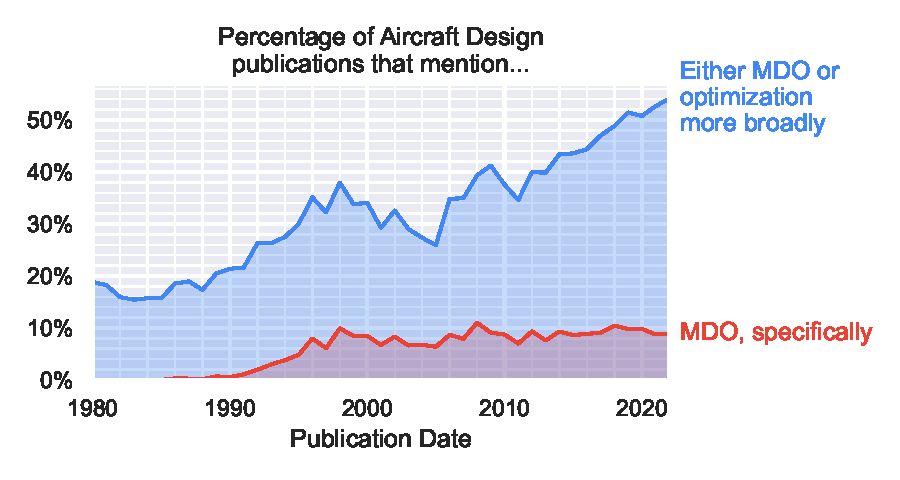
\includegraphics{../figures/mdo_citation_counts}
        \caption{Prevalance of optimization-related keywords in academic literature with the keyword ``aircraft design''. Data from Google Scholar; includes industry-standard texts such as AIAA journals and conference proceedings. MDO-specific keywords (red line) include any of: ``multidisciplinary design optimization'', ``MDO'', and ``MDAO''. The blue line adds the keyword ``optimization'' to this list.}
        \label{fig:mdo_citation_counts}
    \end{figure}

    Moreover, this statistic alone understates the true magnitude of MDO's impact. Arguably the most pivotal contribution of MDO research to aircraft design has been to catalyze a shift towards an \textit{optimization mindset}: the recognition that optimization is not only a useful tool, but also a principled mathematical framework that can represent complete design problems. Figure \ref{fig:mdo_citation_counts} shows that this mindset is a relatively recent development -- the fraction of aircraft design publications mentioning optimization in any form has tripled since the advent of MDO, reaching a majority share today.

    These optimization-based design processes have shown several benefits when used to augment traditional design methods such as point analyses, parametric surveys, and carpet plots \cite{torenbeek_advanced_2013}. Most obviously, formal optimization methods can lead to improved design results and allow the consideration of many more design variables. Optimization can also help human designers discover clever cross-discipline synergies that might otherwise be overlooked \cite{drela_pros_1998}, and its rigor can reduce the likelihood of biased decisions \cite{torenbeek_advanced_2013}. In cases where designer intuition is exhausted, such as with unconventional configurations, optimization provides a means to identifying useful directions for further exploration \cite{drela_pros_1998}. Torenbeek argues that an optimization-based design process can respond more quickly to unexpected changes in program requirements, whereas manual processes often require substantial redesign effort \cite{torenbeek_advanced_2013}. Finally, the optimization mindset itself has benefits, even beyond the results of an optimization study. for example, discussions about problem formulation (how to translate given requirements into a quantified optimization problem) can help a team of engineers align on design goals and expose subtle discrepancies in perceived requirements\footnote{For example, is the objective to minimize fuel burn, or to maximize range? Is operating cost a quantity that should be strictly capped (a constraint), or instead only penalized (an objective)?}.

    Another important area where MDO research has made significant progress is in defining the relationship between the human designer and the optimizer. The prevailing view in the early days of aircraft design optimization was that optimization would eventually advance to the point that computational tools could yield complete, production-ready designs with minimal human oversight -- as evidenced by encouraging titles such as ``Automating the Design Process'' \cite{heldenfels_automating_1973, heldenfels_automation_1974, vanderplaats_automated_1976}. Over time, this has largely given way to a more balanced view: although the optimization solve itself may be well-served by computational means, this forms only one small part of the larger design process. Inputting the engineer's design intent into the optimizer accurately (``problem specification'') and extracting intuition from the results (``interpretation'') are challenges in their own right, and best addressed by iterative human-computer teams. As described by Drela in a 1998 optimization study \cite{drela_pros_1998}, ``[Engineering optimization] is still an iterative cut-and-try undertaking. But compared to [traditional] techniques, the cutting-and-trying is not on the geometry, but rather on the precise formulation of the optimization problem.''

    When considering this full design process (i.e., from initial requirements to product delivery), the scope of challenges becomes even broader. Indeed, industry adoption of MDO is often limited by non-computational user frictions \cite{salas_framework_1998, gpkit, martins_engineering_2021}. In the present work, we deliberately term these user frictions ``costs'', borrowing optimization nomenclature to emphasize that minimizing these frictions is an implied part of the objective function of any optimization-driven design process. Figure \ref{fig:birds_eye_view} summarizes a variety of design literature to present a holistic view of this complete process as applied to aircraft design \cite{torenbeek_advanced_2013, martins_engineering_2021, yang_observations_2009, torenbeek_synthesis_1976, roskam_airplane_1989, nicolai_fundamentals_2010, salas_framework_1998}. Frictions that a designer may experience from a computational optimization framework at each step are shown in \textcolor[HTML]{BB5045}{red}.

    \begin{figure}[h]
        \centering
        \ifdraft{}{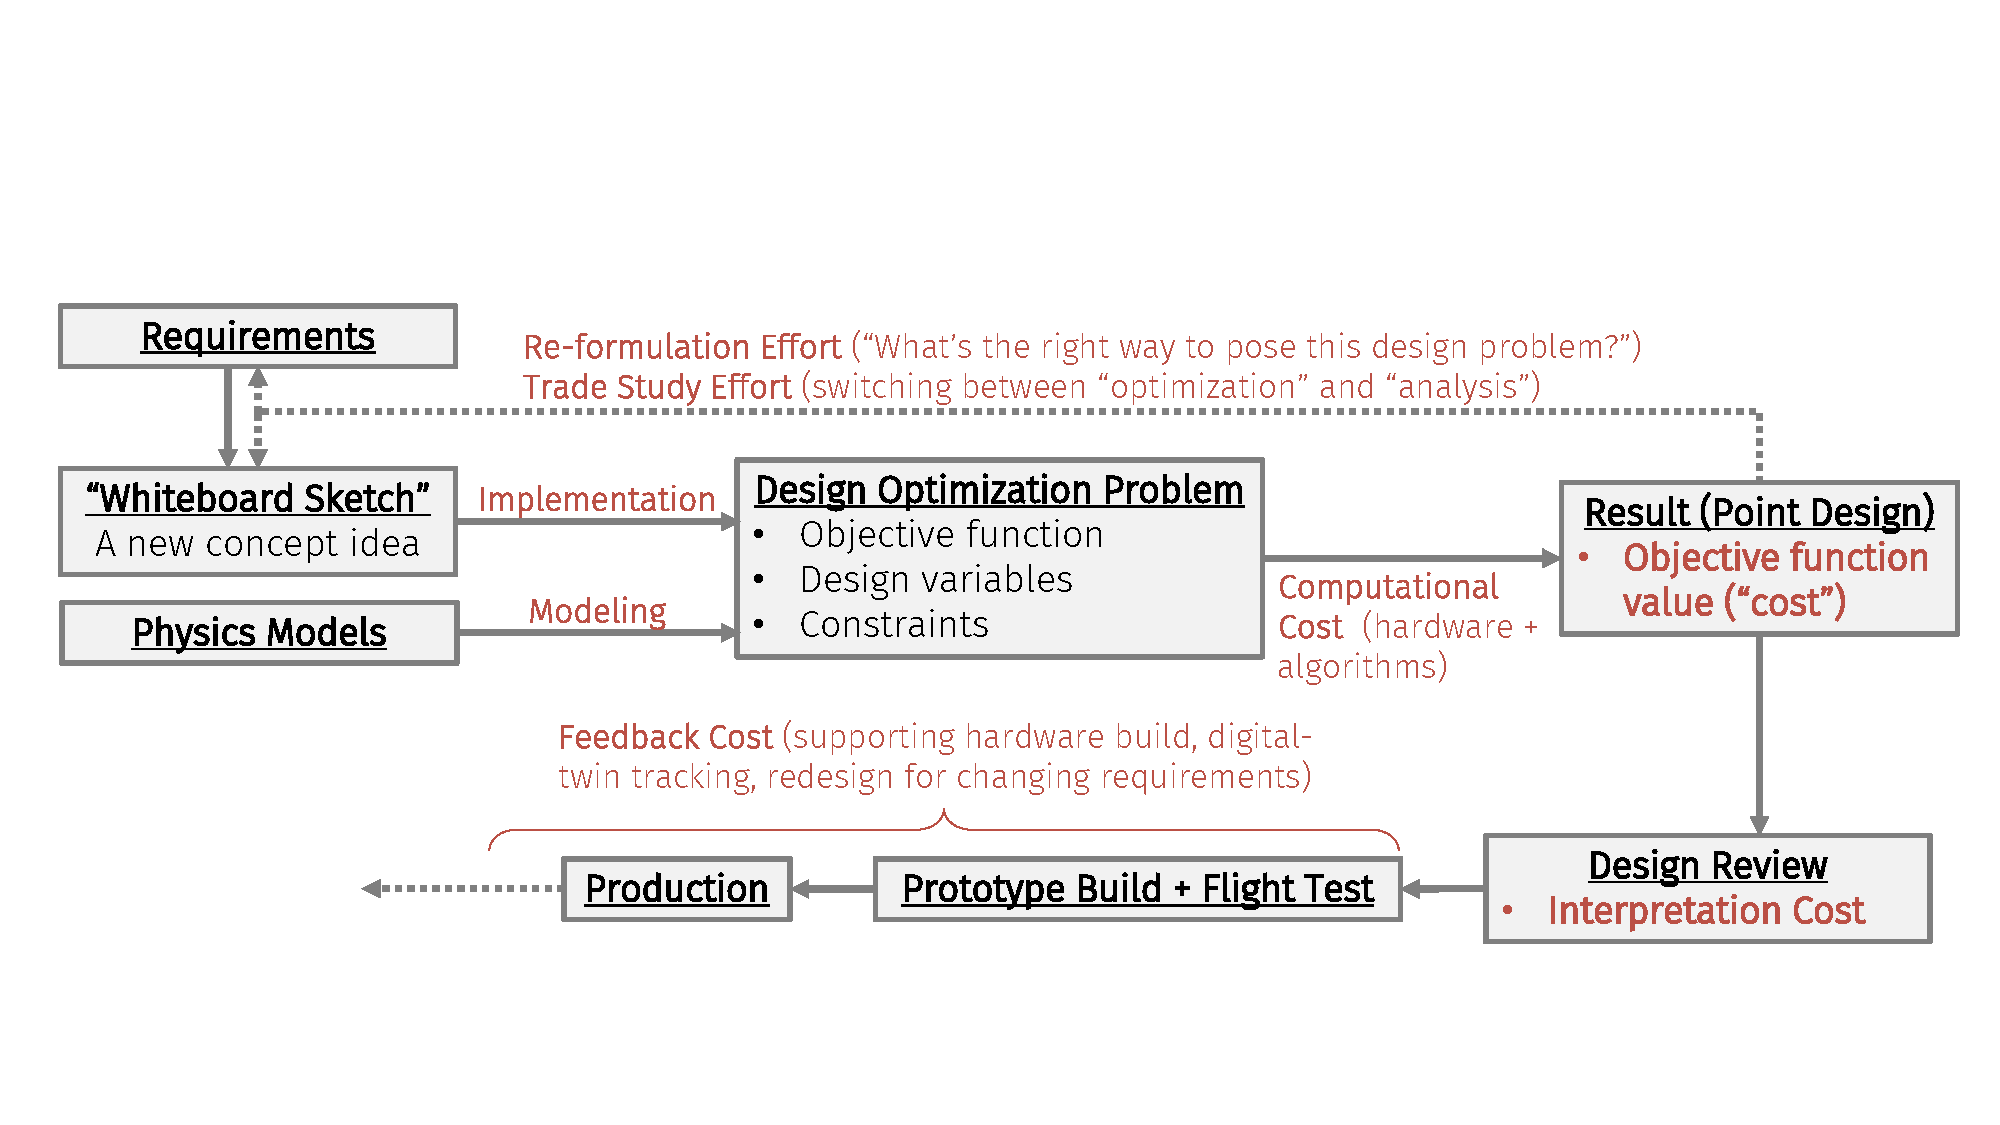
\includegraphics[width=\textwidth]{../figures/design_optimization_process_birds_eye_view}}
        \caption{A high-level overview of the optimization-driven design process, as applied to aircraft design. ``Costs'' (user frictions to be minimized) associated with each step are shown in \textcolor[HTML]{BB5045}{red}.}
        \label{fig:birds_eye_view}
    \end{figure}

    In the aircraft design process model of Figure \ref{fig:birds_eye_view}, the initial point of departure is a set of high-level requirements \cite{torenbeek_synthesis_1976, torenbeek_advanced_2013}. The first design step is to develop a set of candidate concepts (``whiteboard sketches''), a qualitative and configuration-focused process that largely leverages designer creativity and experience \cite{yang_observations_2009, roskam_airplane_1989}. Concepts and the associated requirements are then translated into a formal mathematical design optimization problem consisting of an objective function, design variables, and constraints. Physics models are invoked as needed to support this process; this modeling process incurs a cost that depends on the modeling flexibility of the chosen MDO paradigm \cite{sharpe_aerosandbox_2021}. The optimization problem is then solved, which incurs a computational cost and yields a point design.

    This process of mapping potential concepts to problems and problems to optimized point designs is often iterative. Even for expert users, it is rare that a design optimization process will fully reflect design intent on the first attempt \cite{drela_pros_1998}. In addition, post-optimality studies may be used to assess performance robustness to off-design conditions. The total time required to close this re-formulation loop is a critical driver of how the human interacts with the MDO tool, as it directly rate-limits how much design exploration can be performed.

    For a practical aircraft development program, however, this is only the beginning. The point design must survive external validation and design review by a team of subject-matter-experts; the cost of this process is a direct function of the tools an MDO framework supplies to aid result interpretability. Even beyond this, in prototyping, flight testing, production, and deployment, the design process still imposes framework requirements. For example, an analysis and optimization framework that supports a wide range of modeling fidelities has the potential to can smoothly transition from a conceptual design tool to a digital thread \cite{niederer_scaling_2021, singh_engineering_2018}. Likewise, a design tool can be used during the production process to support manufacturing decisions, such as whether an unexpected change in a component supplier still produces a feasible design with desired margins.

    The remainder of this chapter will discuss some of the most important advances in design optimization research, and how these advances can reduce the costs incurred at various steps of this holistic process.

    \subsection{Two Directions: ``Wide'' vs. ``Deep'' MDO}
    \label{sec:wide_vs_deep}

    Before proceeding further, it is important to clarify the scope of aircraft design optimization problems that are of interest in this thesis, as the definition of ``MDO'' is somewhat overloaded. More precisely, the modern field of MDO can be decomposed into two related but distinct subfields which have developed different strategies and mindsets to address different design needs. Figure \ref{fig:mdo_overloaded_term} illustrates this distinction, showing how the term ``MDO'' can refer to separate tasks at different stages of the aircraft design process.

    \begin{figure}[h]
        \centering
        \ifdraft{}{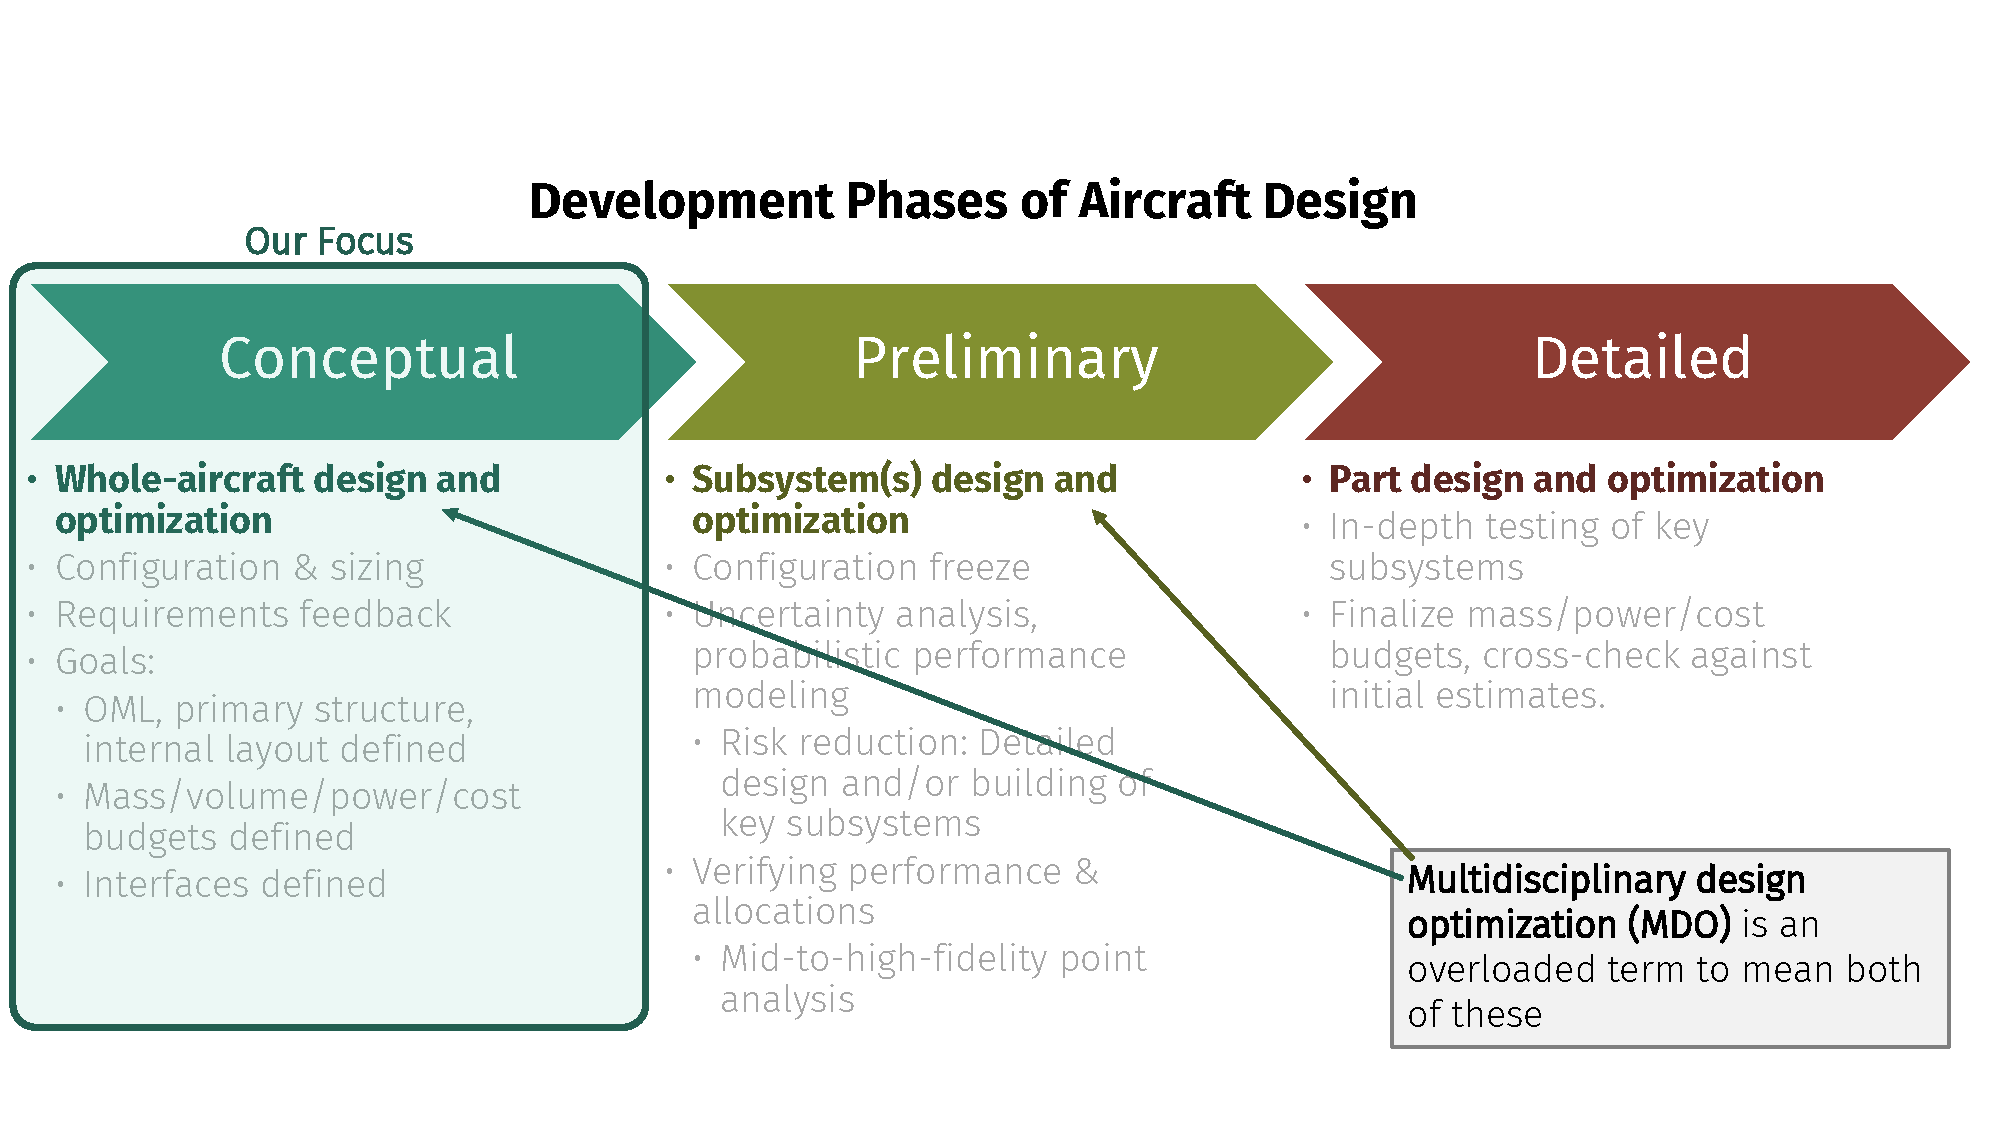
\includegraphics[trim=0cm 1.1cm 0cm 3cm, clip, width=\textwidth]{../figures/mdo_overloaded_term}}
        \caption{Multiple definitions of the term ``multidisciplinary design optimization''. Here, conceptual, or ``wide'' MDO is contrasted against preliminary, or ``deep'' MDO.}
        \label{fig:mdo_overloaded_term}
    \end{figure}

    The first subfield, and the subject of the present work, is that of \textbf{conceptual}, or \textbf{``wide'' MDO}. This is essentially a formalization of the conceptual sizing problem and typically involves casting a wide net to capture as many first-order dependencies as possible. The intended use case is often clean-sheet design of a complete aircraft, and the end goals are often initial identification of strong design drivers and assessment of concept feasibility. Sensitivity analysis is also a key desired output of a wide MDO process. Frameworks that tend to specialize on this class of wide MDO problems are TASOPT \cite{drela_tasopt_2010} and GPkit \cite{gpkit}.

    These goals requires an enormous breadth of models to be considered, as practical aircraft designs are shaped by an enormous number of constraints that do not appear in first-principles performance analysis (e.g., the Breguet range equation). For example, a drag reduction of the vertical stabilizer is of little interest if engine-out performance constraints preclude certification; likewise, a more efficient engine is of little interest if acoustic constraints preclude customer acceptance. This need for analysis breadth can lead to design problems with many hundreds of models spanning anywhere from five to twenty relevant disciplines. To illustrate this breadth, consider the following non-exhaustive list of example disciplines that might be included:

    \begin{multicols}{2}
        \begin{itemize}[noitemsep]
            \item Aerodynamics
            \item Structures and weights estimation
            \item Propulsion
            \item Power systems and thermal management
            \item Flight dynamics (trim, stability, and control)
            \item Internal geometry and packaging
            \item Mission design (concept of operations) and trajectory optimization
            \item Takeoff and landing field length analysis
            \item Certifiability, safety, and engine-out performance
            \item Life-cycle emissions
            \item Cost modeling and manufacturability
            \item Acoustic signature
            \item Ride quality
            \item Survivability and stealth
        \end{itemize}
    \end{multicols}

    Each of these disciplines might include dozens of submodels \cite{cruz_weight_1989, torenbeek_synthesis_1976, torenbeek_advanced_2013, drela_tasopt_2010}. To keep problems tractable despite their large scope, these models are typically low-fidelity; often, they are either derived from first principles physics with appropriate simplifications or regressions to statistical data. Despite the reduced accuracy of these models, they fulfill two critical functions. First, they apply \textit{optimization pressure} to steer the optimizer towards realistic designs, often in subtle, interdisciplinary ways. For example, increasing fuselage length requires increased landing gear length and mass to maintain a proper takeoff rotation angle, reducing the attractiveness of such design changes. Secondly, these low-fidelity models provide information on which constraints might be active near the optimum, allowing computational resources to be devoted to fidelity improvement only where it is needed. Often, these wide MDO problems are posed as large single-level optimization problems, which allows the large number of cross-disciplinary constraints to be computationally represented in a shared namespace \cite{hoburg_geometric_2014}.

    The second subfield of MDO is that of \textbf{preliminary}, or \textbf{``deep'' MDO}. Here, the goal is often to provide detailed design refinement of a very close initial guess. Because the low-hanging fruit has often been picked by this stage, the design problem is often more local in nature, and the number of models is typically smaller than in wide MDO. Likewise, continued improvement from a good initial guess requires high-fidelity models, since the objective function tends to be relatively flat near the optimum and hence highly sensitive to model inaccuracy. For example, RANS-based CFD\footnote{Reynolds-averaged Navier-Stokes; Computational fluid dynamics} models are often used for aerodynamics, at significant cost: optimization runtimes of 1,000 to 100,000 CPU-hours are not uncommon \cite{kenway_multipoint_2014}. To maintain tractability, relatively few disciplines are considered -- often only aerodynamics and structures. The intended use case is often detailed design of a single component or subsystem, such as a wing. Due to computational challenges that tend to be more prevalent in high-fidelity models (e.g., PDE-constrained optimization, adjoint-based gradients, numerical stiffness of models, and convergence of models that use iterative solvers), the subfield of ``deep'' MDO has placed a large focus on MDO architectures that allow multi-level decomposition of the original optimization problem \cite{martins_multidisciplinary_2013}. Frameworks that tend to specialize on this deep MDO subfield are MACH-Aero \cite{he_aerodynamic_2018}, and, to some extent, OpenMDAO \cite{gray_openmdao_2019}.

    While both subfields share broad similarities and provide useful design insight, they are fundamentally attacking different problems: wide MDO is aimed at clean-sheet conceptual design, while deep MDO tends to aim at detailed refinement of a close initial design. Historically, this schism became increasingly apparent roughly in the 1990s and 2000s, as various research groups began ``spending'' their increasing computational budgets in different ways: either model breadth or model depth. Examples of wide MDO research efforts in the time since this divergence include PASS \cite{antoine_framework_2005} by Kroo, TASOPT \cite{drela_tasopt_2010} by Drela, and various GPkit-based \cite{hoburg_geometric_2014} aircraft design codes. Modern ideas around deep MDO research can trace their origins to high-fidelity adjoint-based aerodynamic shape optimization studies by Alonso, Martins, and other contemporaries \cite{alonso_pymdo_2004, martins_coupledadjoint_2005, choi_multifidelity_2008}.

    \subsection{Advances in Optimization Algorithms}

    The current academic state-of-the-art for MDO paradigms has largely centered on two approaches: gradient-based methods with analytical gradients, and disciplined optimization methods. The former tends to be more popular in deep MDO applications, while the latter tends to be more popular in wide MDO applications; however, exceptions exist. These two existing approaches are discussed in turn below. Pros and cons of these existing approaches, as compared to the proposed new paradigm, are summarized in Table \ref{tab:paradigm_comparison} of the subsequent chapter and discussed fully in Appendix \ref{chap:paradigm_comparison}.

    \subsubsection{Gradient-Based Methods with Analytical Gradients}

    Gradient-based optimization offer fundamental scaling advantages over gradient-free methods, and are hence preferred for large-scale design optimization when model characteristics allow \cite{lyu_benchmarking_2014, martins_engineering_2021}. The effectiveness of gradient-based methods is highly contingent on the speed and precision of gradient calculations. To illustrate this, Kirschen and Hoburg show that gradient-based optimization gives inadequate performance on even modest engineering design problems if simple finite-differencing is used \cite{kirschen}. Likewise, Adler et al. show that the inaccuracy of finite-differenced gradients can prevent accurate optimization \cite{adler_cfd_2022}.

    Because of these considerations, a leading academic approach to gradient-based MDO involves manually supplying exact analytical gradients to the optimizer for each submodel. Frameworks like OpenMDAO and MACH-Aero \cite{gray_openmdao_2019} provide example implementations of this manual-gradients approach, forming the basis for several interesting case studies \cite{yildirim_performance_2021, brelje_multidisciplinary_2021, openaerostruct, bons_highfidelity_2020}. Although this paradigm is most often applied to deep MDO problems, it has been applied to wide MDO problems in examples such as OpenConcept \cite{brelje_multidisciplinary_2021} and OpenAeroStruct \cite{openaerostruct}.

    \subsubsection{Disciplined Optimization Methods}

    Another MDO paradigm that has become popular in recent years is that of disciplined optimization methods, borrowing nomenclature from Grant \cite{grant_disciplined_2006}, Agrawal \cite{agrawal_disciplined_2019}, and Boyd \cite{boyd_tutorial_2007, boyd_convex_2004}. These methods are considered \textit{disciplined} as they impose a strict set of rules on the optimization problem formulation, which allows the optimizer to make assumptions about the problem structure (such as convexity, or log-convexity). These assumptions allow the optimizer to make more efficient use of computational resources and provide guarantees of global optimality. Geometric programming in particular has proven to be a useful disciplined MDO paradigm for aircraft design applications, as originally observed by Hoburg \cite{hoburg_geometric_2014}. GPkit \cite{gpkit, hoburg_geometric_2014, kirschen}, a framework that demonstrates this geometric programming concept targeting engineering design applications, has led to successful case studies such as the Jungle Hawk Owl aircraft \cite{jho} and Hyperloop system studies \cite{gpkit}.

    \subsection{Advances in Design Optimization Practice}
%     complexity -- motivating the idea of general-purpose \textit{MDO frameworks} to address this as opposed to problem-specific codes

    % Multipoint

    % UQ


    % Importance of geometry - CPACS, Haimes work
    A recent notable shift in aircraft design optimization perspectives has been a renewed focus on geometry representation and parameterization. For example, Haimes and Drela \cite{haimes_construction_2012} contended in 2012 that ``constructive solid geometry (CSG) is the natural foundation for [aircraft design optimization]''. This publication extended prior work by Lazzara, Haimes, and Willcox \cite{lazzara_haimes_willcox_multifidelity_geometry_2009} that introduced the concept of ``multifidelity geometry''. Together, these works advocated for accurate 3D outer mold line representations from the earliest stages of conceptual design, with degenerate representations of this central geometry used to drive individual discipline analyses. Furthermore, they recognized the fundamental limitations of general-purpose (e.g., Parasolid-based) CAD tools in aircraft design optimization: because aerospace geometries tend to use complex, lofted surfaces, the resulting CAD models can be brittle with respect to parameter changes. This observation, along with later developments such as differentiable discretization techniques \cite{esp}, led to renewed research on how aircraft geometry should be parameterized for optimization. For example, in recent years aircraft-specific geometry tools like OpenVSP \cite{mcdonald_open_2022} and Engineering Sketch Pad \cite{esp} have been developed for design optimization workflows, a trend that arguably stems from this line of research.
% TODO transition
    In a broader sense, another notable area where computational methods for aircraft design have long made inroads to industry is in inverse design tools. (An example of successful industry adoption in aerodynamics the inverse approach used by the XFoil airfoil design code \cite{drela_xfoil_1989} and others \cite{liebeck_blendedwingbody_1998} to recover a shape from a specified pressure distribution.) Like optimization methods, these inverse methods can aid designers because they offer fundamentally different capabilities than traditional design methods (e.g., carpet plots). While traditional methods focus on the ``forward problem'' (design $\rightarrow$ performance), inverse methods and optimization methods both focus on the ``inverse problem'' (performance $\rightarrow$ design). Drela \cite{drela_pros_1998} shows that this more-manual inverse approach can lead to more robust designs than optimization, if the user is not familiar with the risks of an improperly-specified optimization problem.

%    \subsection{Emerging Trends and Opportunities}
%
%
%    It would be remiss to discuss the last decade of optimization advances (and in particular, the growing recognition of the \textit{interpretability problem} of large-scale computational tools) without discussing the explosion of interest in machine learning. Learning is inherently an optimization problem to develop a generalized regressor model from given observations.
%
%    Indeed, a major criticism of generative AI in the present day is that it yields results that appear plausible on the surface level but may be deeply flawed in ways that are difficult to detect. In many ways, it is not the incorrectness, but rather the difficulty of detecting incorrectness that poses the largest threat of breaching trust. This is a problem that is not unique to AI, but rather is a fundamental challenge of large-scale computational tools in general.

    \subsection{Advances in Numerical Methods}

    In the past two decades several notable scientific computing techniques have matured to the point of practical use in engineering design optimization. Two of the most significant advances are automatic differentiation and automatic sparsity detection, which are discussed in detail below. A review focusing on these two techniques is available in work from Andersson et al. \cite{casadi} and Rackauckas \cite{rackauckas_generalizing_2021}. Review of several other notable scientific computing advances, such as GPU-accelerated computing, probabilistic programming, deep learning, and uncertainty quantification, are omitted here for brevity. A wider review of state-of-the-art scientific computing techniques is available from Lavin et al. \cite{lavin_simulation_2022}

    \subsubsection{Automatic Differentiation}

    Here, we review literature on \textit{automatic differentiation}, an advanced technique borne out of the machine learning community that fundamentally accelerates gradient-based optimization algorithms. A comprehensive modern survey is available by Baydin et al. \cite{baydin_automatic_2018}. A 2008 textbook by Griewank and Walther \cite{griewank_evaluating_2008} provides a more in-depth review of the mathematical foundations of automatic differentiation.

    Gradient-based optimization methods are computationally bottlenecked by the cost of computing gradients \cite{lyu_benchmarking_2014, martins_engineering_2021}. Existing state-of-the-art workflows have users manually derive and implement highly-efficient gradients for each model, but this is time-consuming and thus impractical for early-stage design. Automatic differentiation (AD) is an efficient and accurate way to automatically compute the gradients of a function \textit{as represented in code} at runtime. In many cases, the computational complexity of this technique is fundamentally better than traditional approaches like finite-differencing; Griewank provides concrete upper bounds on the worst-case time complexity \cite{griewank_automatic_1988}.

    Automatic differentiation exploits the fact that any function can be broken into a series of simple mathematical operators, which can then be represented as a computational graph. As a practical matter, this computational graph is often created by tracing program execution with an overloaded numerics library. This graph construction process is illustrated in Figure \ref{fig:computational-graph}. The chain rule can then be applied to this graph to compute the Jacobian of the function. Various modes of automatic differentiation effectively allow this Jacobian construction to occur either column-by-column (forward-mode) or row-by-row (reverse-mode) \cite{casadi, jax, martins_engineering_2021}; depending on the shape of this Jacobian, one strategy may be enormously more efficient than the other.

    \begin{figure}[H]
        \centering
        \centerline{\begin{tikzpicture}[
    auto,
    node distance=0.8cm
]
    \tikzstyle{var} = [
    draw = c1, fill = c1!20,
    minimum height = 1cm,
    rectangle, rounded corners, thick,
    text width = 1cm, text centered,
    ]

    \tikzstyle{num} = [
    var,
    draw=c1!15!gray, fill=c1!15!gray!20
    ]

    \tikzstyle{func} = [
    var,
    draw = c2, fill = c2!20,
    ellipse
    ]

    \tikzstyle{line} = [draw, thick, ->, shorten >=2pt, shorten <=2pt]

    \node[text centered, align=center, text width = 5cm](label) {
        A computational graph for $f(a,b) = 2ab + \sin(a)$
    };

    \node[below=of label](start) {};

    \node[var, left=of start](a) {$a$};
    \node[num, right=of a](2) {$2$};
    \node[func, below=of 2](times1) {$\times$};
    \node[var, below=of a](b) {$b$};
    \node[func, below=of times1](times2) {$\times$};
    \node[func, below=of times2](sum) {$+$};
    \node[func, left=of times2](sin) {$\sin()$};
    \node[num, right=of sum, text width = 1.5cm](f) {$f(a, b)$};

    \begin{scope} [every path/.style=line]
        \path (a) -- (times1);
        \path (2) -- (times1);
        \path (times1) -- (times2);
        \path (b) -- (times2);
        \path (times2) -- (sum);
        \path (a) edge[out=-135, in=135] (sin);
        \path (sin) -- (sum);
        \path (sum) -- (f);

    \end{scope}

\end{tikzpicture}}
        \caption{A computational graph, as would be used for automatic differentiation. Reproduced from \cite{sharpe_aerosandbox_2021}.}
        \label{fig:computational-graph}
    \end{figure}

    Advances in automatic differentiation (and in particular, combining this with GPU computing) are largely responsible for the revolution of practical advances in machine learning in the past decade \cite{baydin_automatic_2018}. Rackauckas in 2021 \cite{rackauckas_generalizing_2021} states: ``[Automatic differentiation] has become the pervasive backbone behind all of the machine learning libraries. If you ask what PyTorch or Flux.jl is doing that’s special, the answer is really that it’s doing automatic differentiation over some functions.'' The goal is that similar practical advances can be brought to bear in engineering design optimization, a field that has similar potential to benefit from this scientific computing technique.

    \subsubsection{Automatic Sparsity Detection and Jacobian Coloring}

    The process of gradient computation for optimization can be further accelerated if the sparsity of the constraint Jacobian is known a priori. This is because sparsity can guarantee structural independence of multiple columns\footnote{or rows, if using reverse-mode automatic differentiation} of the Jacobian, so the respective elements of the Jacobian can be evaluated simultaneously. Sparse Jacobians arise frequently in the modeling of physical systems, especially multidisciplinary ones \cite{lambe_extensions_2012}; because of this, this represents a significant opportunity in engineering design. The process of reducing the number of Jacobian evaluations by simultaneously evaluating independent columns is known as \textit{Jacobian compression} and is illustrated in Figure \ref{fig:jacobian_coloring}. To enable compression, independent columns of the Jacobian must be grouped. This process is known as \textit{Jacobian coloring}, referencing mathematical similarities to the graph coloring problem if the Jacobian's sparsity pattern is represented as a bipartite graph \cite{gebremedhin_efficient_2009}. This coloring problem does not readily admit exact solution for Jacobian sizes of interest; however, Gebremedhin et al. provide a comprehensive review of graph coloring heuristics that work well in practice \cite{gebremedhin_what_2005}. Martins and Ning provide a more concise summary that contextualizes this process around the backdrop of design optimization \cite{martins_engineering_2021}.

    \begin{figure}[H]
        \centering
        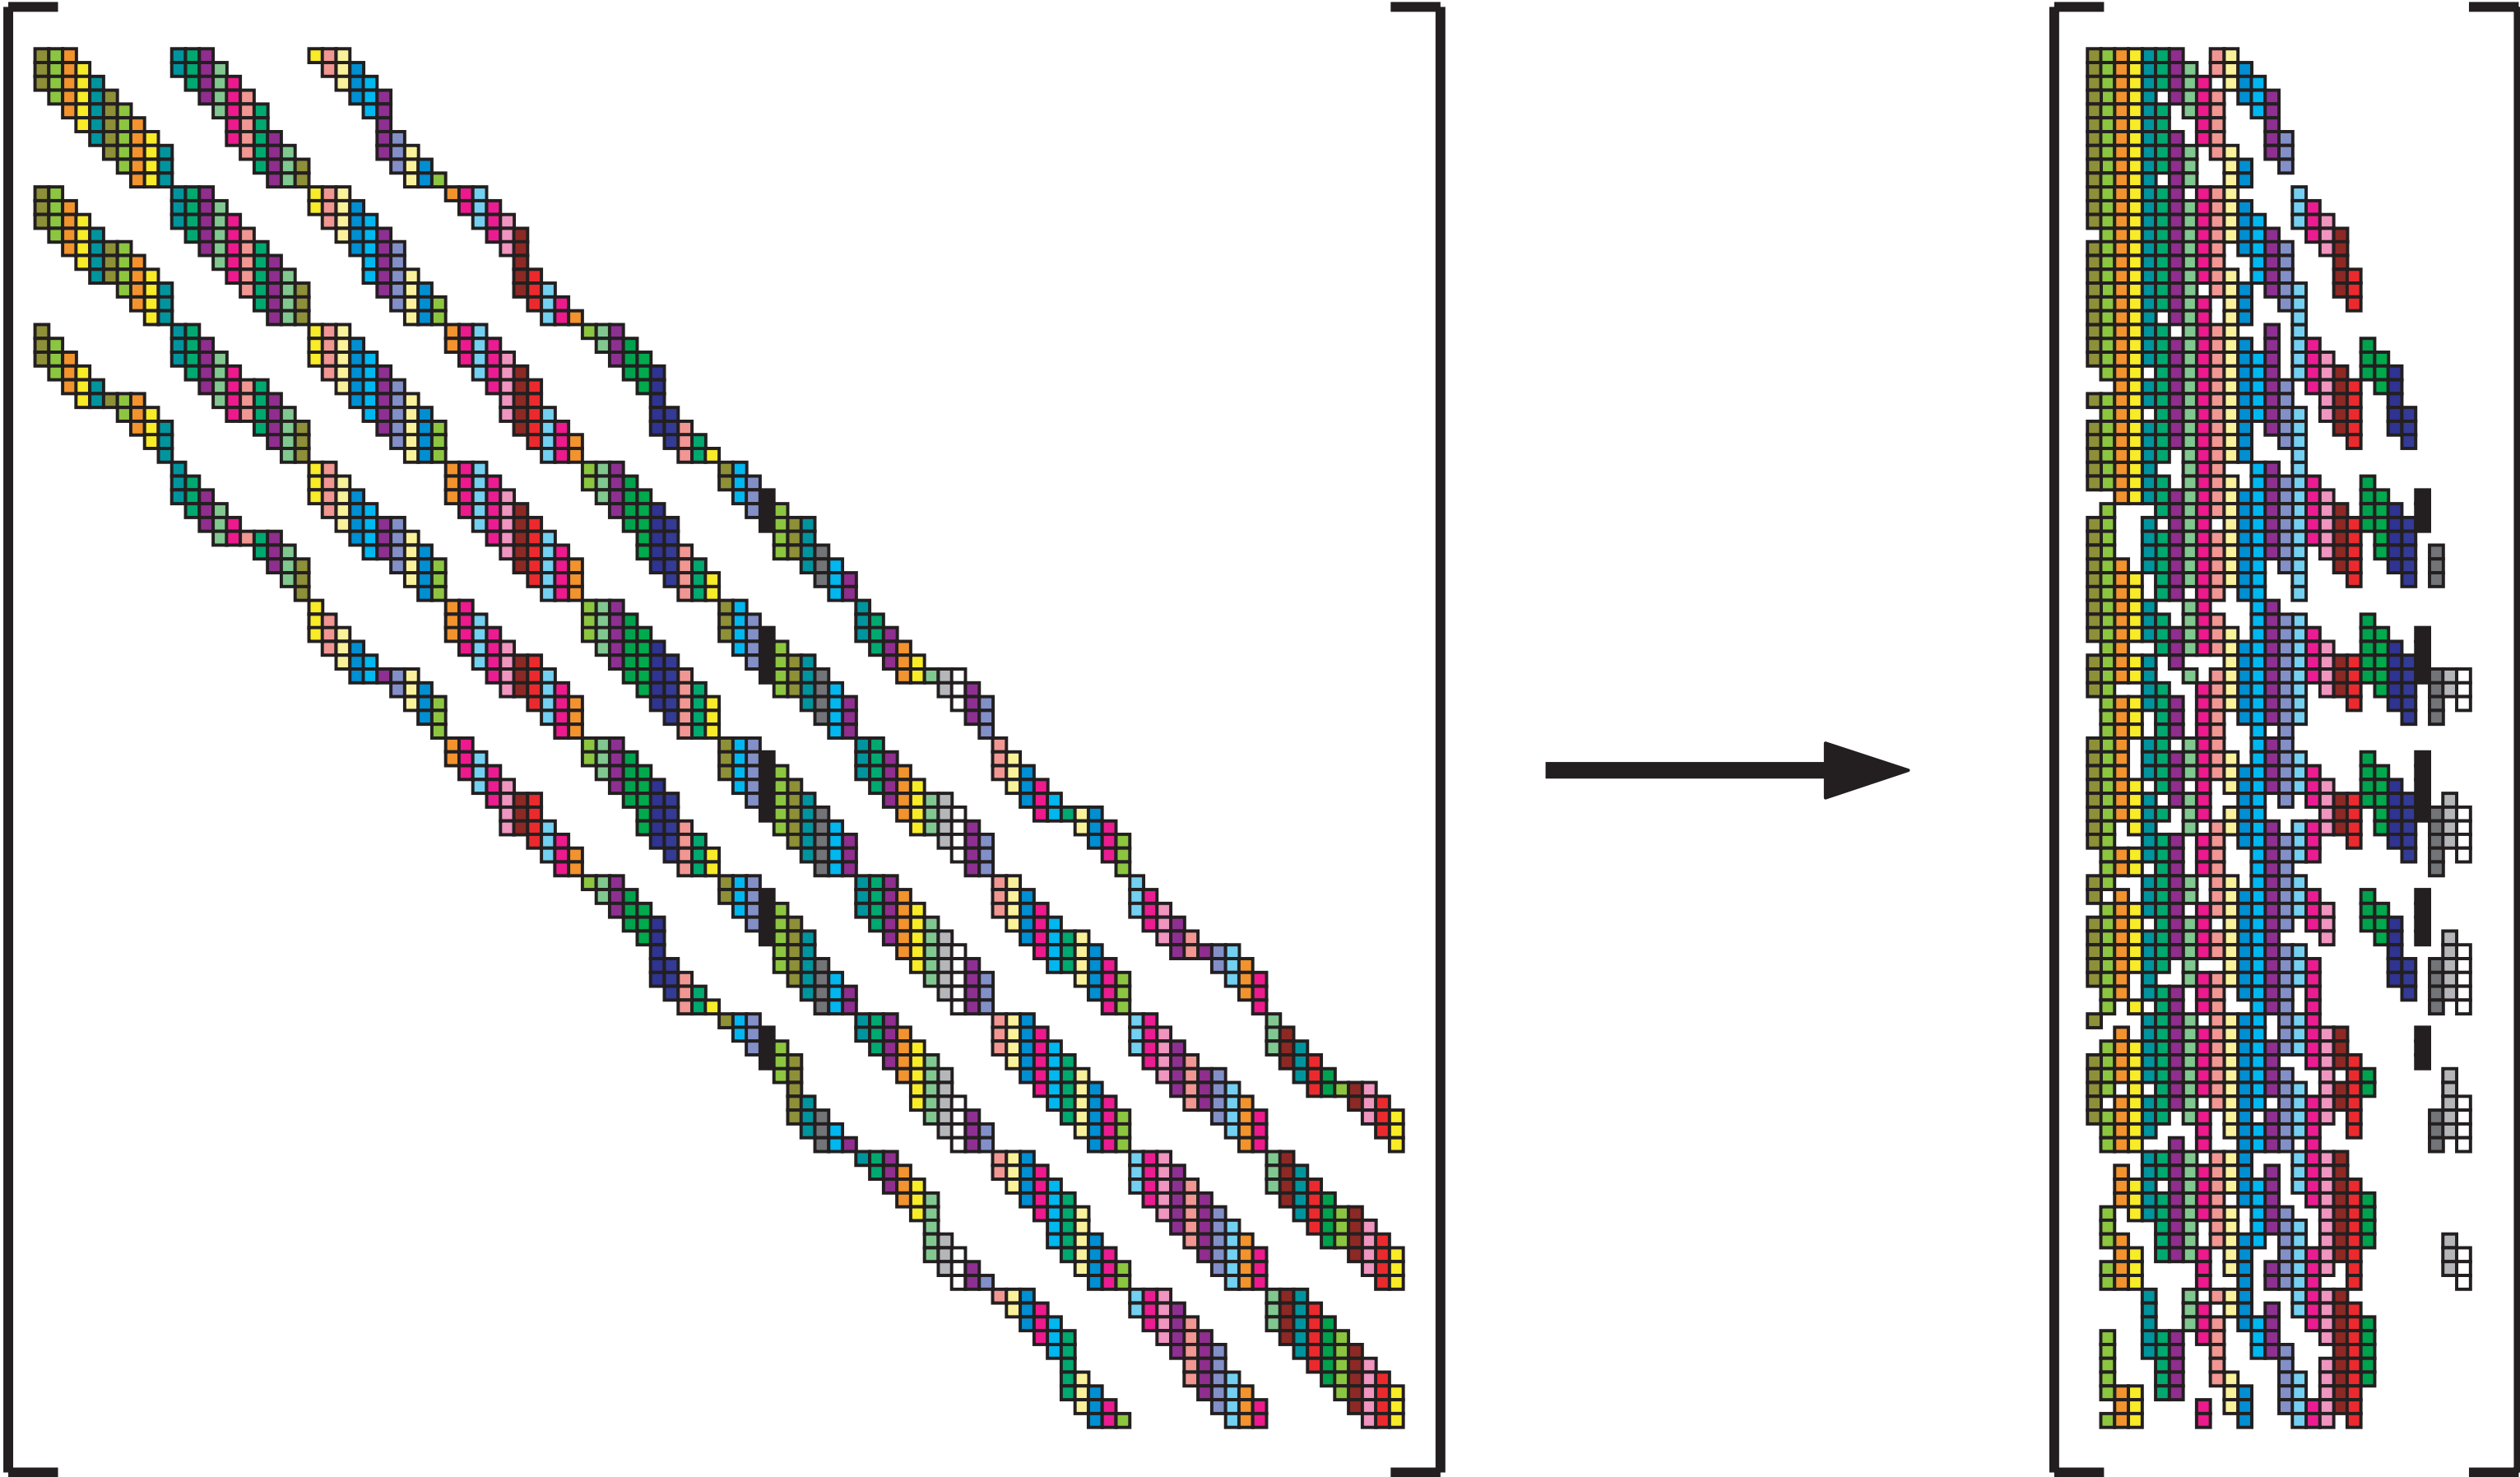
\includegraphics[width=\textwidth]{../figures/gebremedhin_2005_figure}
        \caption{A sparse Jacobian can be evaluated more quickly by simultaneously evaluating derivatives that are structurally independent, a process known as Jacobian coloring and compression. On the left of the figure is the original Jacobian; on the right is its compressed form. Figure reproduced from Gebremedhin et al. \cite{gebremedhin_what_2005}}
        \label{fig:jacobian_coloring}
    \end{figure}

    Before Jacobian coloring and compression can be performed, the sparsity pattern of the Jacobian must be known. This is a nontrivial task and an area of active research, with the major complications summarized by Rackauckas \cite{rackauckas_generalizing_2021}. In recent years, automated sparsity detection has enabled automatic construction of sparsity patterns using a tracing approach that is quite similar to that of automatic differentiation. This bypasses many of the potential edge-case failure modes that can occur when trying to infer sparsity purely by inspecting the dense Jacobian, such as conditional branching or cancellation. Indeed, the same computational graph can be used for this process, making this a computationally-efficient addition to a code base that already leverages automatic differentiation. Andersson et al. \cite{casadi} provide an example implementation of this automated sparsity detection within the CasADi framework. Gowda et al. provide a more complete review on state-of-the-art methods in automated sparsity detection \cite{gowda_sparsity_2019}, with state-of-the-art implementations of this by Ma et al. \cite{ma_modelingtoolkit_2021}.

    \afterpage{\FloatBarrier}

    \section{Motivations for Improving Industry Access to Design Optimization}

    This thesis focuses on improving the accessibility of advanced optimization methods for industry practitioners, with a particular focus on techniques applicable to conceptual (``wide'') MDO for aircraft. This focus is motivated by several factors.

    \subsubsection*{Motivation 1: A Majority of Performance, Risk, and Cost is Committed Early}

    First, the vast majority of the performance of the final design is determined by early-stage conceptual design decisions. This can manifest in both a positive and a negative sense: after the conceptual design is frozen, most design opportunities cannot be captured later and most design regrets cannot be fixed. Figures \ref{fig:motivation_1a} and \ref{fig:motivation_1b} illustrates the two sides to this coin with practical examples.

    The first example, shown in Figure \ref{fig:motivation_1a}, reproduces conceptual design work on the D8 ``Double Bubble'' transport aircraft configuration by Drela \cite{drela_development_2011, drela_simultaneous_2010}. Among other technology improvements, the configuration leverages a strategy of improving passenger loading/unloading speed, which allows for a reduced cruise Mach number while retaining comparable door-to-door travel times (a surrogate for passenger acceptance). This synergistic strategy creates a feedback loop which dramatically reduces fuel burn compared to designs that are optimized on a per-component decomposition basis. For example, one of Drela's main observations from a 2010 work \cite{drela_simultaneous_2010} is that ``multi-discipline optimization considerably increases the fuel savings compared to single-discipline optimization.''

    \begin{figure}[H]
        \centering
        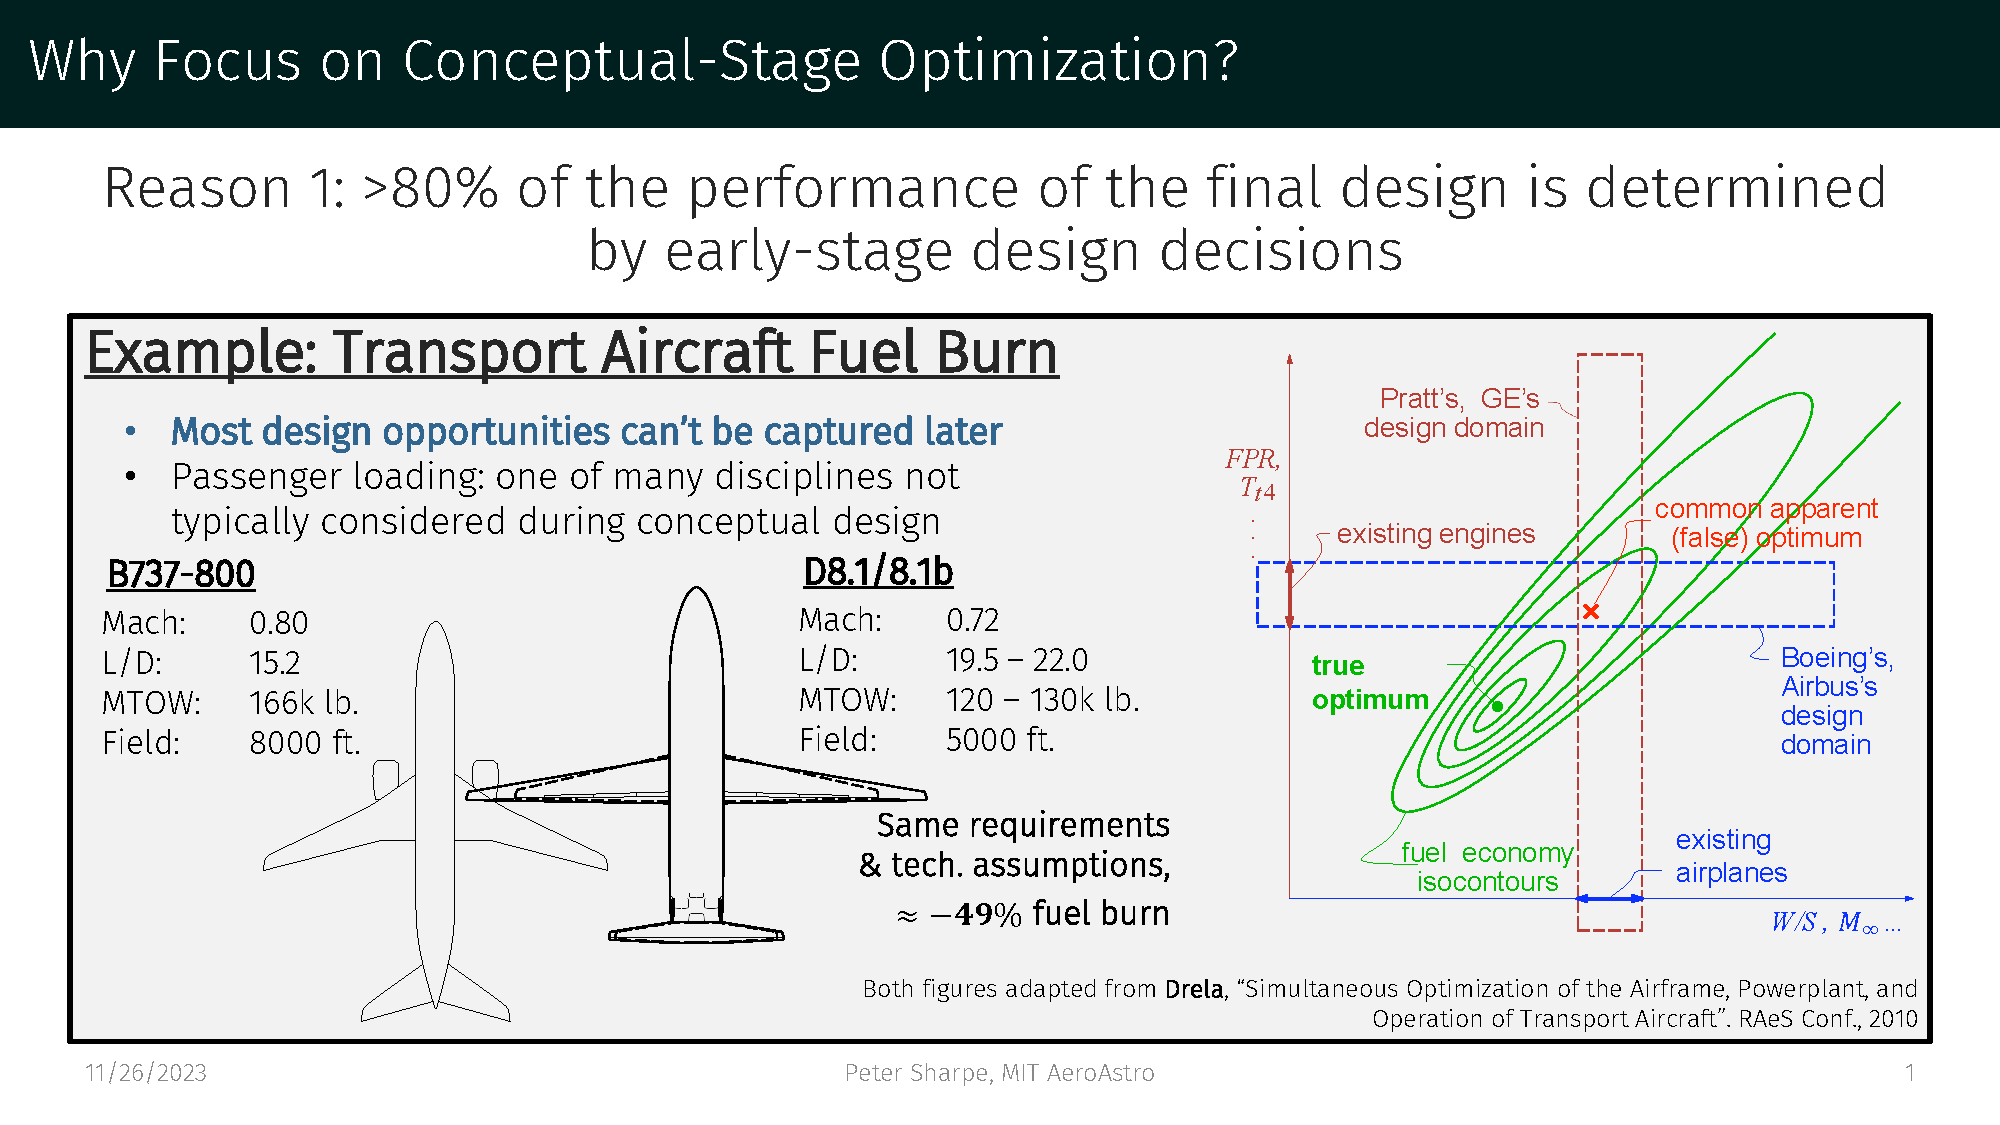
\includegraphics[page=1,trim=1cm 1.3cm 1cm 5cm, clip, width=\textwidth]{../figures/motivation_for_conceptual_MDO_focus.pdf}
        \caption{In an example from Drela \cite{drela_development_2011}, large potential fuel savings are available for transport aircraft if cross-discipline couplings are considered early in the conceptual design process. Figure elements reproduced from Drela \cite{drela_simultaneous_2010}.}
        \label{fig:motivation_1a}
    \end{figure}

    In a second example, shown in Figure \ref{fig:motivation_1b}, the other side of this effect is shown. Here, various electric vertical-takeoff-and-landing (eVTOL) aircraft design concepts are compared. Given the significant energy limitations of battery-powered aircraft, much of the focus of eVTOL conceptual design in the early 2010s was on traditional unit-economics performance metrics of range and payload fraction. However, as these vehicles begin to approach FAA certification and initial deployment, significant regulatory concerns have been raised about the community noise impact of such vehicles. Aeroacoustic noise, to first order, is a strong function of propulsor disk loading and blade tip speed \cite{marte_review_1970}, factors which require substantial redesign to modify later. Hence, manufacturers have had varying levels of difficulty in adapting to this renewed focus on acoustics, as this metric is largely locked in from conceptual design decisions made many years ago.

    \begin{figure}[H]
        \centering
        \includegraphics[page=2,trim=1cm 1.3cm 1cm 5cm, clip, width=\textwidth]{../figures/motivation_for_conceptual_MDO_focus.pdf}
        \caption{Design regrets may arise if conceptual MDO studies do not include all relevant disciplines. This example of contemporaneous eVTOL designs assesses aeroacoustic noise, a factor that is largely determined by conceptual design decisions made many years prior. Although noise is not traditionally included in conceptual aircraft design relations, it is crucial for certification and acceptance. Thus, including many disciplines in conceptual design -- even non-traditional ones, like acoustics -- is key for avoiding major downstream design regrets.}
        \label{fig:motivation_1b}
    \end{figure}

    \afterpage{\FloatBarrier}

    \subsubsection*{Motivation 2: New Technologies Reignite a Need for Early-Stage Design Exploration}

    A second motivation for the focus on conceptual MDO is that recent technological shifts have significantly expanded the aircraft design space compared to previous eras, calling for new tools to aid in down-selecting design concepts.

    As a first example shown in Figure \ref{fig:motivation_2a}, miniaturization and uncrewed aircraft have opened up new trade spaces to explore, calling for renewed focus on first-principles early-stage design optimization. These micro-drone aircraft are able to take more risks with exotic designs, due to shorter design cycles, lower cost, and reduced certification and safety risks. New disciplines, such as packaging and folding considerations, drive new trades -- in many cases, volume allocation trades can be as sensitive as mass fraction trades in conventional aircraft. Another new trade is that of size, weight, and power (SWaP) allocations to autonomy and onboard computing. For small air vehicles, flight computer power requirements can equal or exceed propulsive power, creating new incentives that tilt the design space towards control simplicity \cite{sudhakar_balancing_2020}. New missions, particularly those that are ``dull, dirty, and dangerous'' are enabled by uncrewed aircraft with attritable design and cost optimization. Finally, physics scaling laws, like the square-cube law and transitional Reynolds numbers, cause unique concerns for small-scale aircraft that warrant first-principles conceptual design optimization.

    \begin{figure}[H]
        \centering
        \begin{subfigure}[t]{0.22\textwidth}
            \centering
            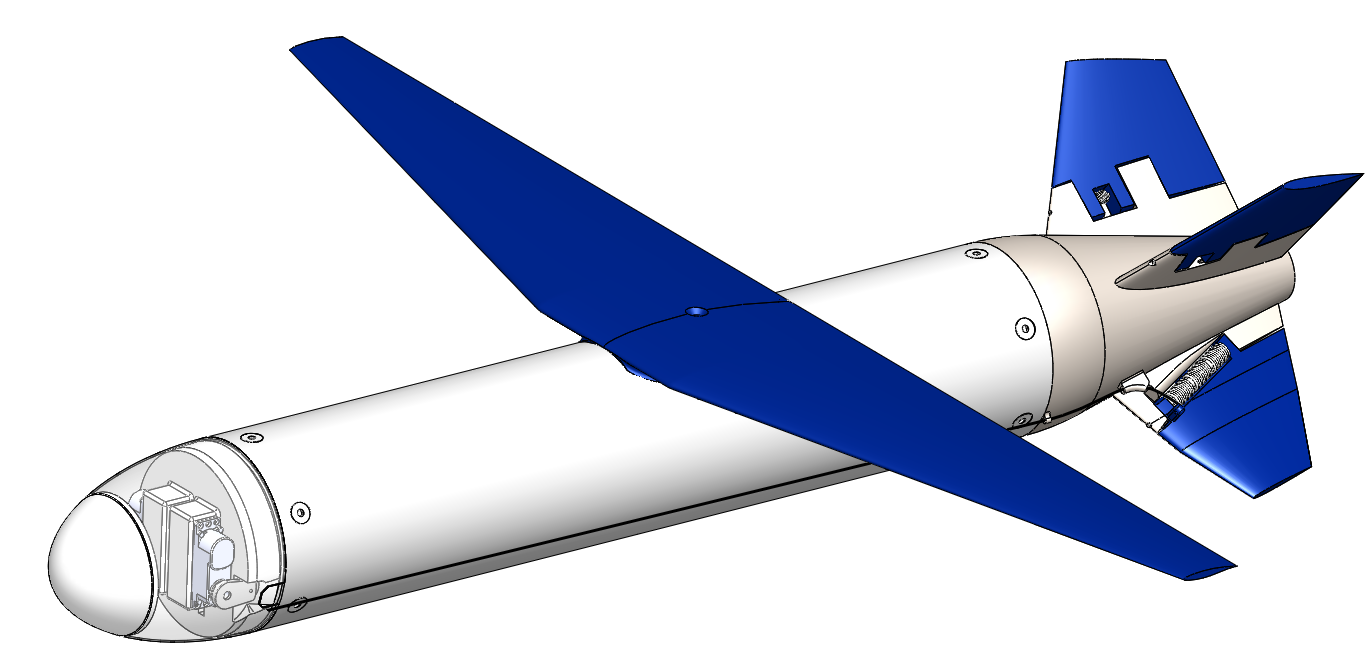
\includegraphics[width=\textwidth]{../figures/drones/firefly.png}
            \caption{MIT Firefly, a Mach 0.8, rocket-propelled micro-UAV \cite{popmech_firefly, mathesius_firefly_2019}}
            \label{fig:firefly}
        \end{subfigure}
        \hfill
        \begin{subfigure}[t]{0.22\textwidth}
            \centering
            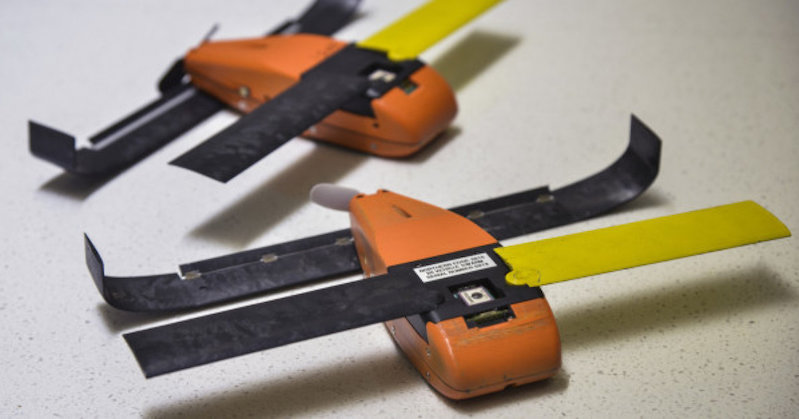
\includegraphics[width=\textwidth]{../figures/drones/perdix.jpeg}
            \caption{MIT Perdix, an air-launched ALE-55-class ISR UAV \cite{tao_design_2012}}
            \label{fig:perdix}
        \end{subfigure}
        \hfill
        \begin{subfigure}[t]{0.22\textwidth}
            \centering

            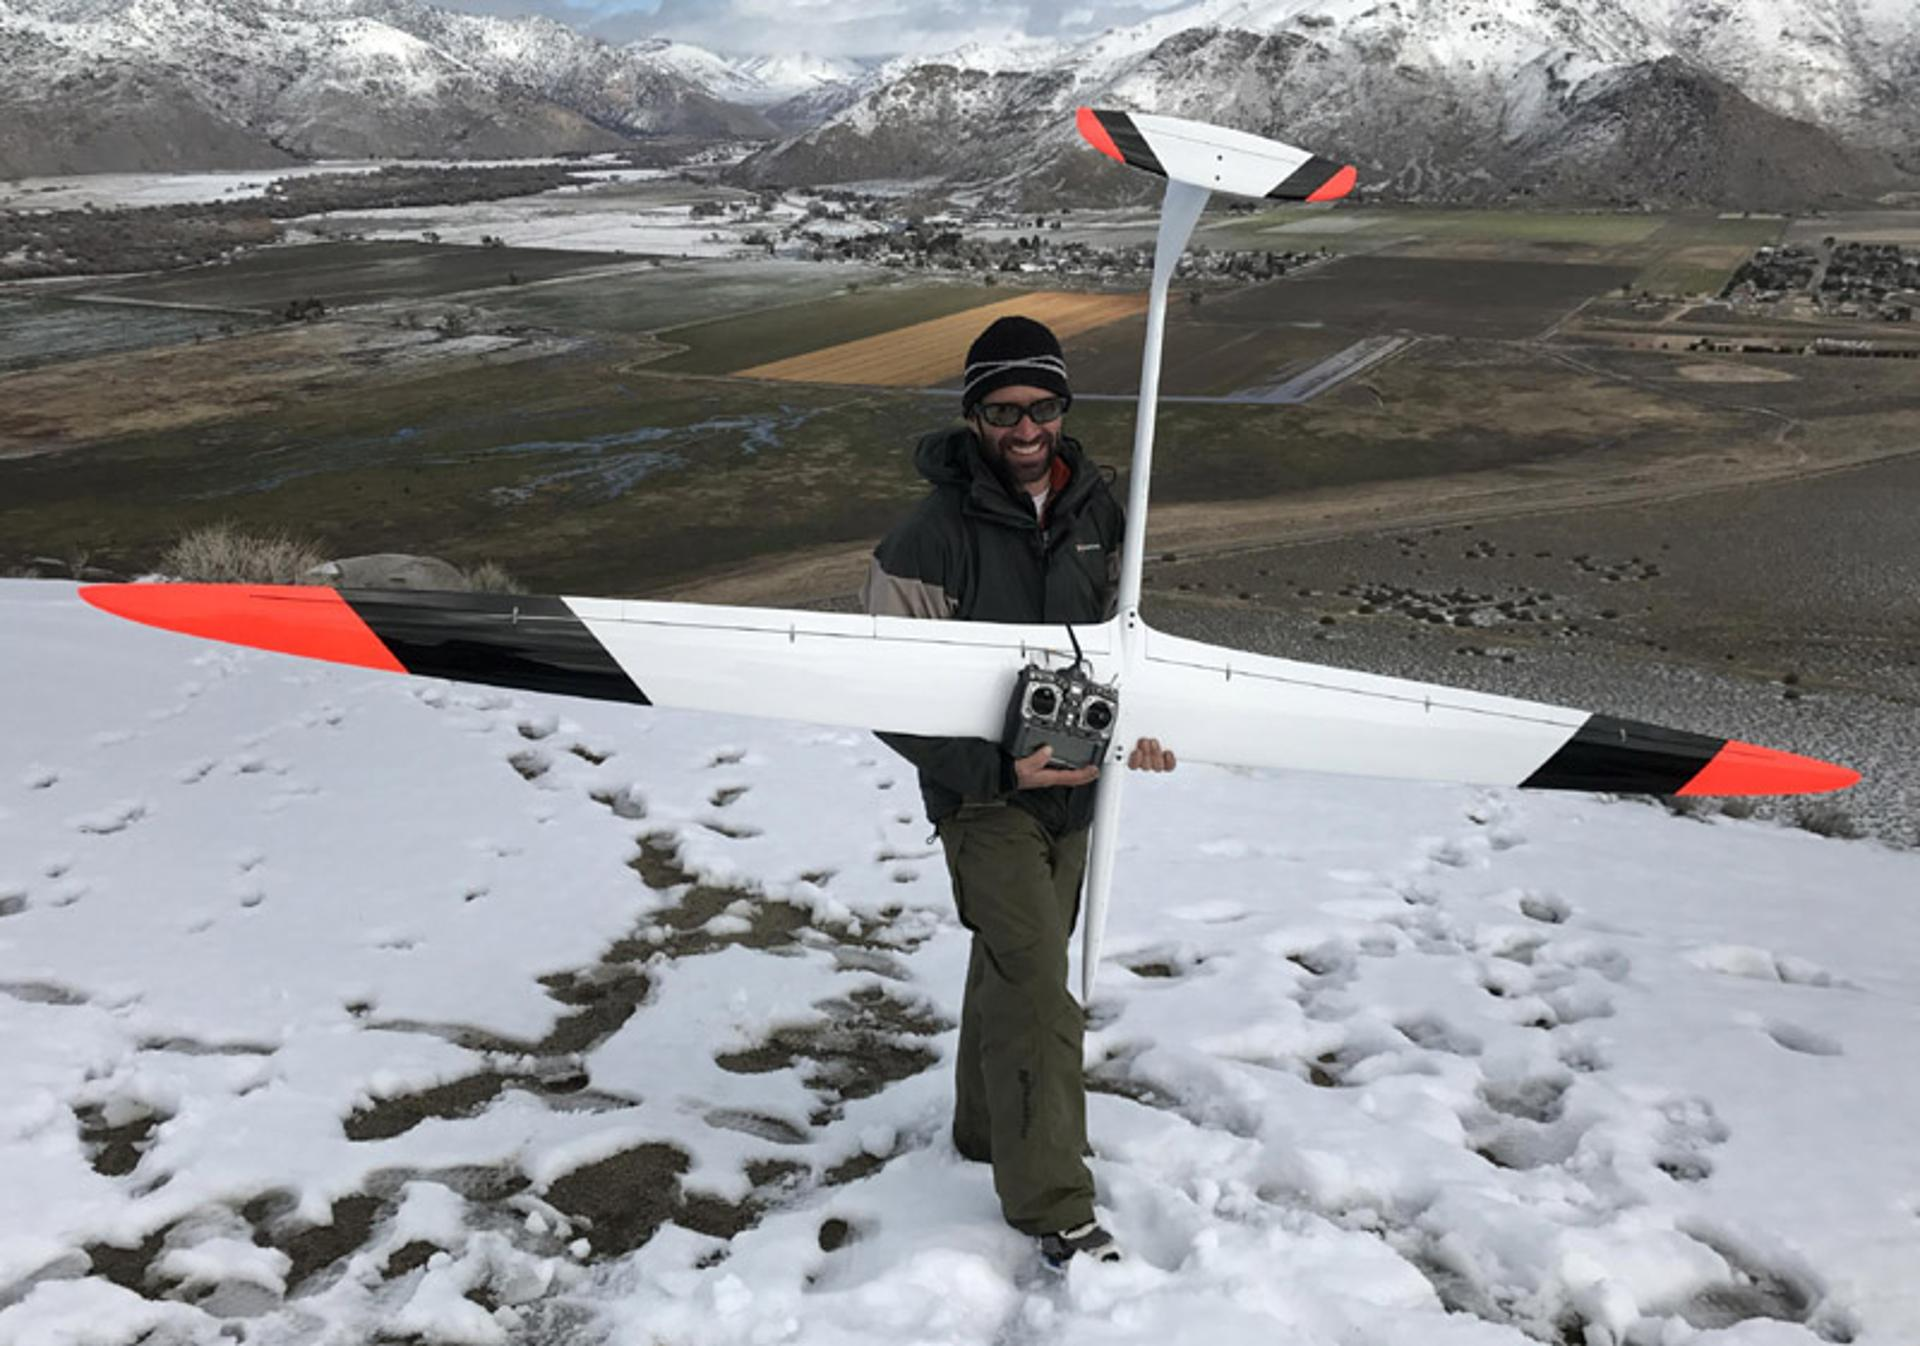
\includegraphics[width=\textwidth]{../figures/drones/transonic_dp.jpeg}
            \caption{Transonic DP, a 545-mph dynamic soaring glider with 100 G turn capability (photo: Spencer Lisenby)}
            \label{fig:transonic_dp}

        \end{subfigure}
        \hfill
        \begin{subfigure}[t]{0.22\textwidth}
            \centering
            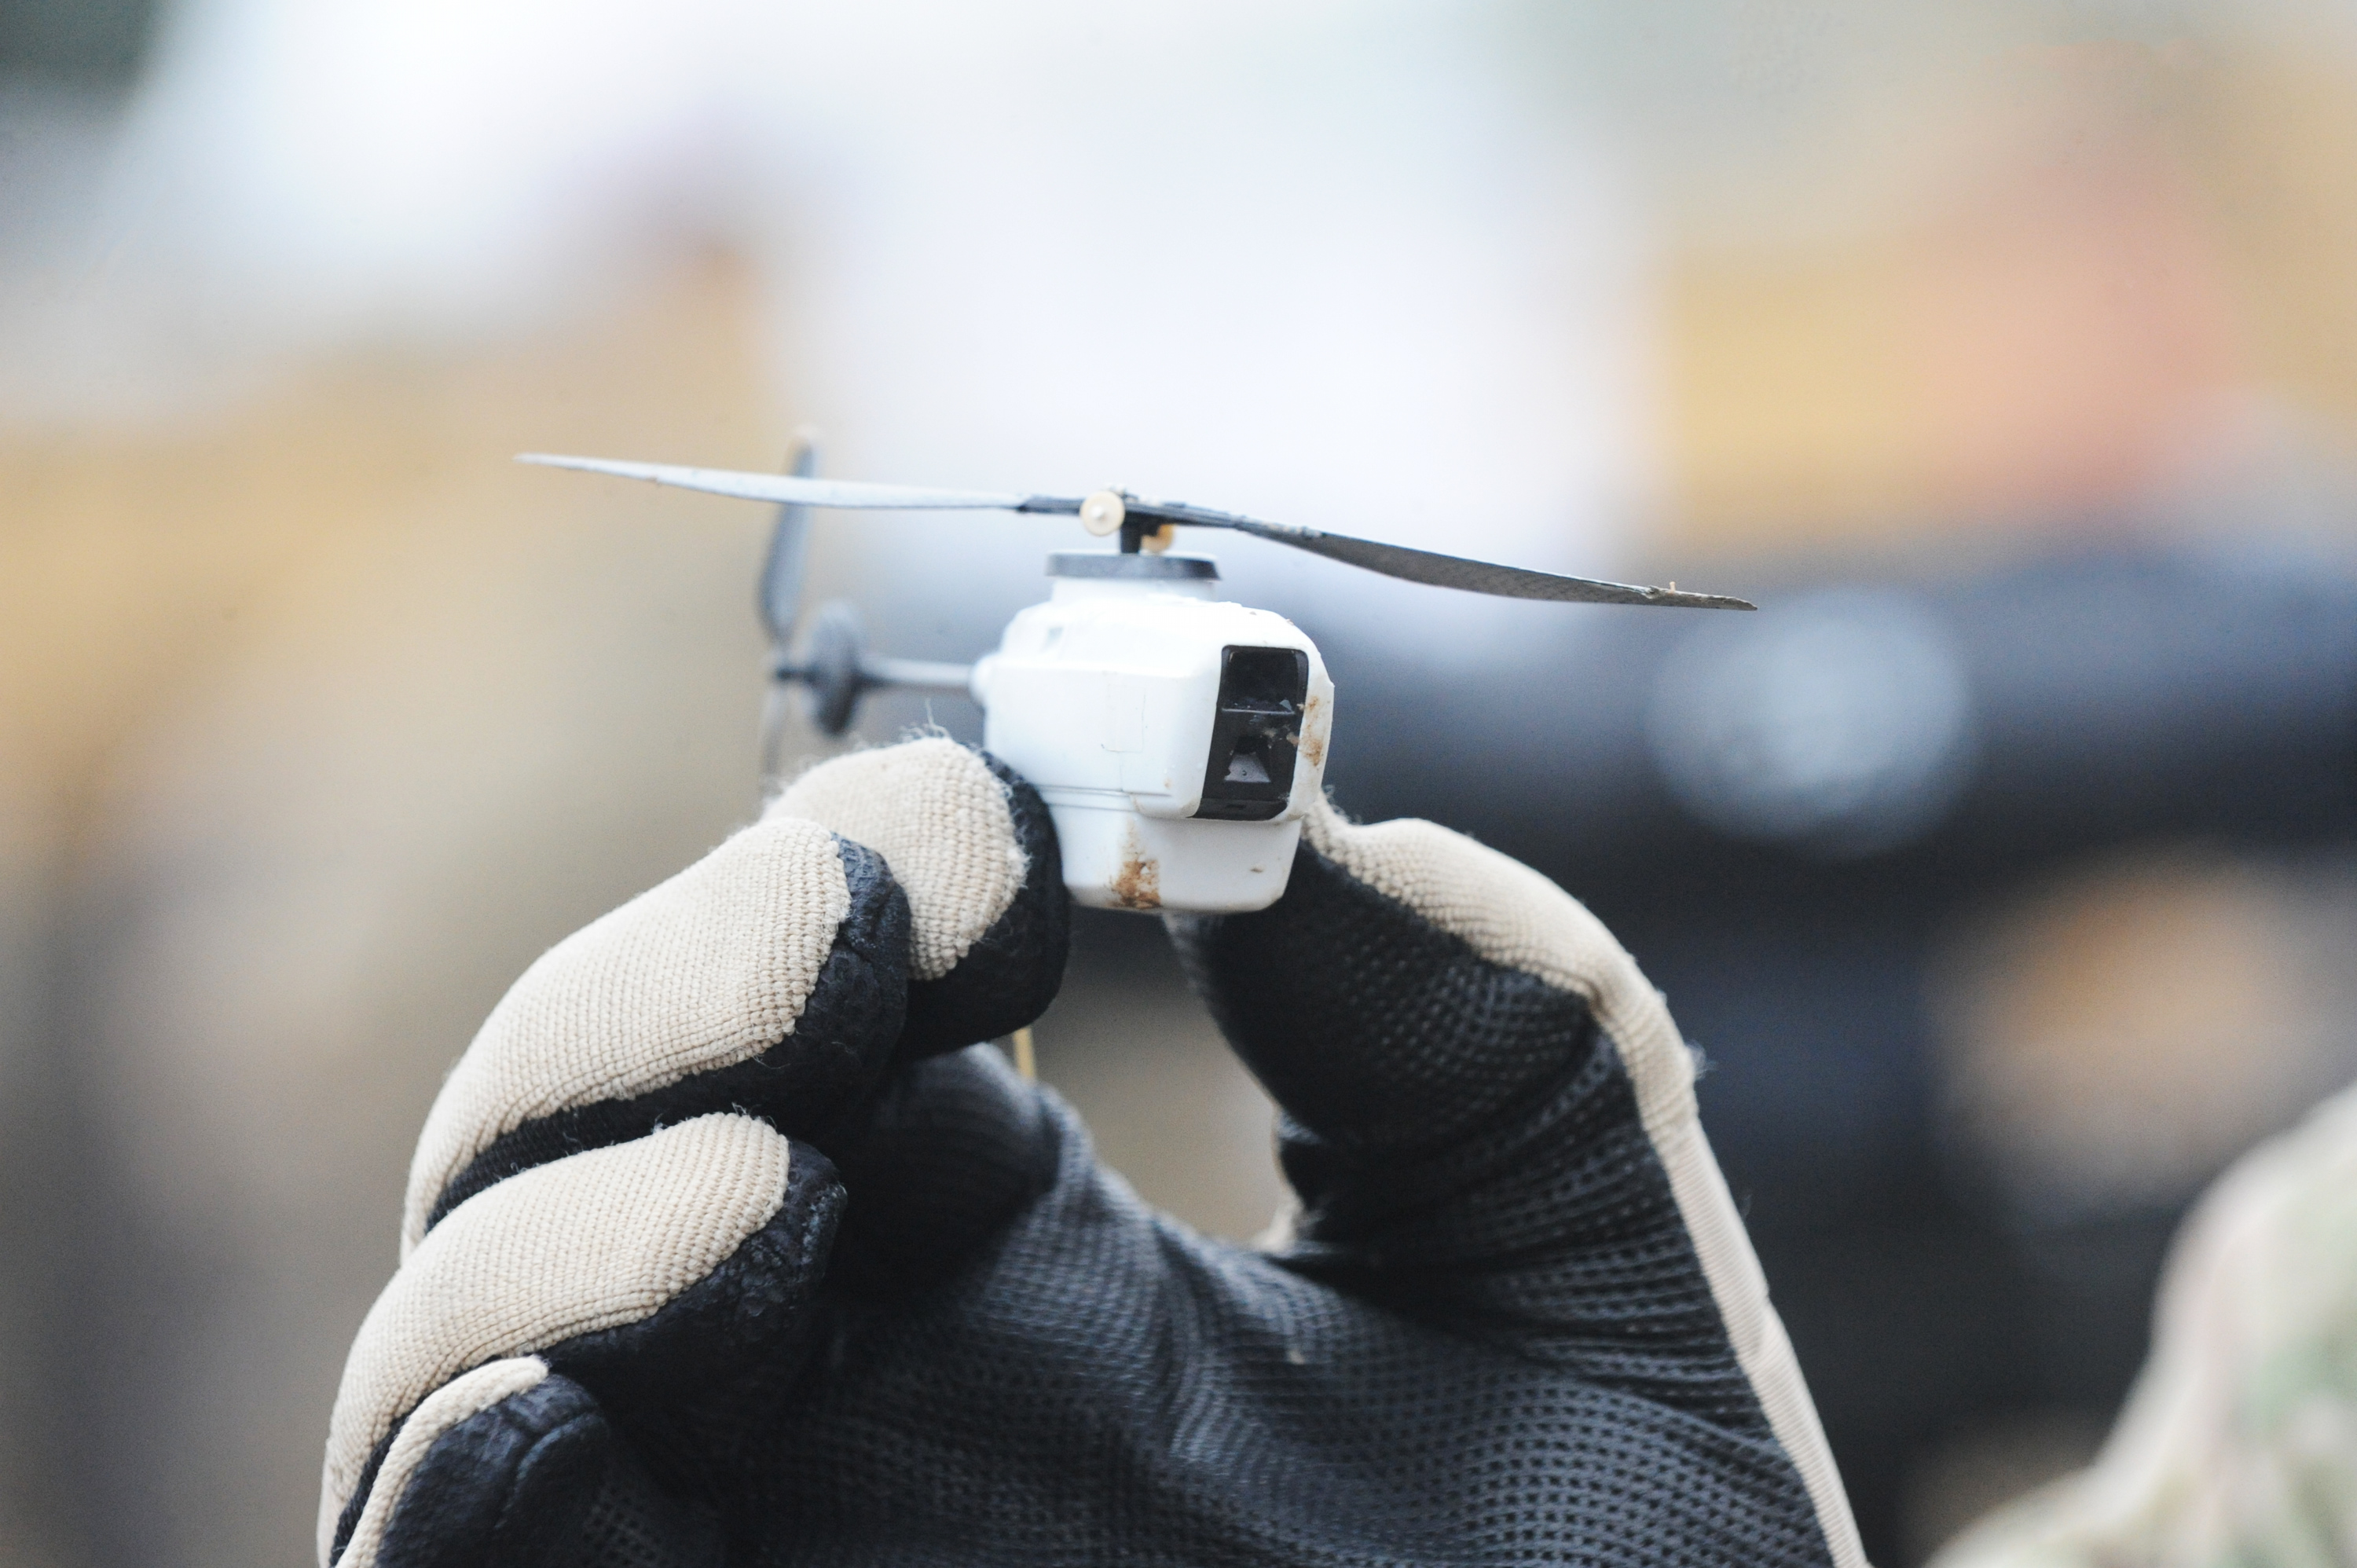
\includegraphics[width=\textwidth]{../figures/drones/hornet.jpeg}
            \caption{Black Hornet Nano, an 18-gram ISR helicopter (photo: Richard Watt/MOD)}
            \label{fig:hornet}
        \end{subfigure}
        \caption{Examples of new design spaces enabled by miniaturization and uncrewed aircraft technology in recent years.}

        \label{fig:motivation_2a}
    \end{figure}

    Another prominent new design space that motivates revisiting first-principles conceptual aircraft design is electric aviation, as shown in Figure \ref{fig:motivation_2b}. Electric propulsion offers a fundamentally different configuration trade space compared to conventional propulsion. In terms of energy storage, modern lithium batteries have realizable\footnote{in other words, after accounting for the generally-higher powertrain efficiencies of electric propulsion due to the lack of a thermodynamic gas cycle} specific energies that are roughly 1/25th that of kerosene, placing extreme sizing demands here. On the other hand, electric motors have excellent specific power across a wide range of size scales, dramatically fewer moving parts, and wider power bands compared to combustion engines. These factors make electric motors far more modular, essentially allowing designers to place propulsors at will -- electric aircraft with eight or more propulsors are not uncommon. The enormous design space that electric propulsion opens up is evident in Figure \ref{fig:motivation_2b}, where the diversity of aircraft configurations is wholly unprecedented compared to other aerospace domains. Part of the value proposition of conceptual MDO is that it can make rigorous design within this large space more tractable.

    \begin{figure}[H]
        \centering
        \includegraphics[page=4,trim=1cm 1.3cm 1cm 5cm, clip, width=\textwidth]{../figures/motivation_for_conceptual_MDO_focus.pdf}
        \caption{Electric propulsion opens up a much larger aircraft configuration space, since electric motors offer higher specific power and modularity than combustion engines. A focus on early-stage conceptual design is critical for down-selecting from this diversity of configuration options. Figure adapted from SMG Consulting \cite{aam_reality_index}.}
        \label{fig:motivation_2b}
    \end{figure}

    \afterpage{\FloatBarrier}

    \subsubsection*{Motivation 3: Design Space Exploration}

    The final and most significant motivation for this thesis' focus on early-stage MDO is that it provides value far beyond merely the point design that results from an optimization study. The true value of conceptual MDO is in determining which questions a design team should be asking. Examples of such questions that might be fueled by a design tool leveraging conceptual MDO are given in Figure \ref{fig:motivation_3}. Though some of these questions can be answered with traditional methods, like post-optimality studies and parameter sweeps, modern conceptual MDO tools can supercharge this to tens, hundreds, or thousands of design variables, allowing for a much more comprehensive exploration of the design space. The inclusion of similarly large numbers of relevant constraints effectively prunes the design space, reining unrealistic designs that a parameter sweep might otherwise yield. This capability is especially important in the early stages of a program, where the design space is often poorly understood and the design team is still developing an intuition for the problem. In this sense, conceptual MDO is a tool for \textit{design space exploration}, not just design optimization.

    \begin{figure}[H]
        \centering
        \includegraphics[page=5,trim=0cm 3cm 0cm 6.2cm, clip, width=\textwidth]{../figures/motivation_for_conceptual_MDO_focus.pdf}
        \caption{Conceptual MDO provides far more utility than just the point design that results from an optimization study. It can help designers develop an intuition for the problem space and determine which questions to ask next. This figure gives examples of such exploratory questions.}
        \label{fig:motivation_3}
    \end{figure}

    \afterpage{\FloatBarrier}


    \chapter{Proposed Contributions and Approaches}
    \label{chap:contributions}

%    \section{The Technical Gap: Practical Limitations of MDO Frameworks in Industry}
%    \label{sec:technical-gap}
%    % TODO whole section
%    The primary remaining explanation, which has become increasingly accepted in the past decade \cite{agte_mdo_2010, torenbeek_advanced_2013, gazaix_industrialization_2017, gpkit}, is that MDO faces a set of related organizational, culture, and practical challenges that must be addressed before widespread industry adoption can occur.
%
%    Summarizing this body of work yields a list of MDO's current major challenges:
%    \begin{enumerate}
%        \item MDO can be time-consuming to set up. As stated by Torenbeek in 2013 \cite{torenbeek_advanced_2013} on contemporaneous MDO tools, ``the MDO methodology can be used at any design stage although its complexity does not justify application in the early conceptual phase.''
%        \item MDO can be time-consuming to run \cite{gpkit}.
%        \item MDO faces interpretability challenges, particularly as problem size grows. If MDO is not interpretable and
%        \item If practitioners are not experienced, it is easy to inadvertently produce designs with poor off-design performance, overly aggressive margins, and violated assumptions \cite{torenbeek_advanced_2013, drela_pros_1998, ozturk_optimal_2021}. This often leads to non-credible designs or program failures.
%        \item Most MDO frameworks are syntactically complex, requiring users to be joint experts not only in aircraft design, but also in applied math and computer science \cite{salas_framework_1998, gpkit, agte_mdo_2010}. This ``expertise barrier'', as termed by Grant \cite{grant_disciplined_2006}, is a severe impediment to widespread adoption among ``users whose focus is the application''.
%    \end{enumerate}
%
%    TODO


%    \subsection*{Current Industry Challenges}

%    Interestingly, many of the challenges identified by early MDO works \cite{kroo_multidisciplinary_1997, ashley_making_1982} are the same ones that the field is grappling with today.

    % Challenges of MDO as an "invariant" over time

%    \cite{salas_framework_1998} % Framework Requirements for MDO Application Development

%    TODO

%    In particular, the challenges of \textit{interpretability} and \textit{reviewability} of large-scale engineering design optimization problems are still largely unsolved.

%    The first two barriers to industry adoption that Kroo identifies can be partially explained by the limited computational power of the time. For example, using higher-fidelity analyses to account for more edge cases or adding more disciplines to address coupled design drivers both may require significantly more computational resources.

%    However, beneath these concerns, and particularly in Kroo's notes about managing complexity, Kroo begins to unearth a more fundamental challenge of practical aircraft design optimization. The utility of an MDO tool is often limited by the human designer's ability to implement, manage, and interpret complexity -- can the results be reviewed and trusted? Indeed, this challenge is not only independent of computational complexity, but often exacerbated by it.


%    This observation that not all challenges cede to Moore's law, while made a fundamental impact on the field's direction. Papers from the 1970s with

%    Contemporaneous publications from leading voices in the field of aircraft design around the time of Kroo's work paint a similar story - expressing optimism about the field's growing potential while highlighting (or in some cases, urging) hesitation by industry practitioners.

    % Practical optimization does not necessarily tend towards integrated design. Barnaby Wainfan, designer of the Facetmobile and Technical Fellow for Aerodynamics at Northrup Grumman: one of the under-appreciated benefits of the "conventional" configuration is that it is \textit{modifiable} -

    The Ph.D. thesis will make five following novel conceptual contributions which to address the technical gap and motivation identified in Chapter \ref{chap:literature}. A concise list of these contributions is given in Section \ref{sec:definition}. Here, we expand upon each of these contributions in detail, discuss intended approaches to making advances here, and discuss the results to date.

    \section{Code Transformation Paradigm}
    \label{sec:code_transformations}

    The thesis will introduce the idea of \textit{code transformations} as a new computational paradigm on top of which an MDO framework can be built. Here, code transformations are defined as a generalized set of computational techniques that intercept the original optimization problem posed by the user (at runtime), apply some improvement based on analysis of the code itself, and then solve a modified optimization problem instead. This encompasses a variety of recent advanced techniques in scientific computing, such as:
    \begin{itemize}[noitemsep]
        \item Automatic differentiation \cite{griewank_automatic_1988}
        \item Automatic sparsity detection \cite{gebremedhin_efficient_2009}
        \item Problem transformations:
        \begin{itemize}[noitemsep]
            \item Auto-scaling \cite{nocedal_numerical_2006}
            \item Log-transformation of variables, constraints, and objectives (similar to geometric programming) \cite{kirschen, agrawal_disciplined_2019}
            \item Redundant constraint elimination
        \end{itemize}
        \item Backend-agnostic programming (CPU/GPU, different math library backends, just-in-time compilation, automatic vectorization and parallelization) \cite{jax}
    \end{itemize}

    The benefit of introducing this abstraction is to recognize that all of these advanced techniques essentially share one major requirement to use: the optimization framework must be able to inspect the actual code driving the design problem. This code inspection is done either via direct source code analysis or by creating a computational graph of the optimization model at runtime. The latter approach, which is called \textit{tracing} in machine learning literature \cite{jax, frostig_compiling_2018, baydin_automatic_2018}, is widely preferred to the former in modern, syntactically-rich languages\footnote{Maclaurin provides a comprehensive discussion of the tradeoffs between these techniques, and why tracing is often preferable in practice \cite{maclaurin_modeling_2016}}. Therefore, for the purposes of this work, \textit{traceability} is effectively synonymous with code transformability.

    If code transformation techniques can be applied to engineering design optimization, they offer order-of-magnitude speedups over the black-box optimization methods that form the vast majority of industry use today \cite{martins_engineering_2021, lavin_simulation_2022}. These achievable speeds are comparable to those of state-of-the-art optimization methods in academia, such as disciplined optimization methods\footnote{such as geometric programming and disciplined convex programming} \cite{grant_disciplined_2006, gpkit, boyd_convex_2004, agrawal_disciplined_2019} and gradient-based methods using user-provided analytic gradients\footnote{sometimes referred to as ``adjoint methods'' in reference to a common method for manually deriving these gradients for more-complex analyses} \cite{gray_openmdao_2019, kenway_effective_2019, innes_don_2019}.

    However, code transformations offer a key advantage over these state-of-the-art methods in that they can be applied \textit{automatically} -- most of the benefits of these advanced techniques can be gained without requiring any additional effort (or mathematical expertise) from the user. This ease-of-use is critical for practicality -- Grant notes that existing paradigms are hamstrung by a ``expertise barrier'' of existing methods, as described by Grant \cite{grant_disciplined_2006}. Table \ref{tab:paradigm_comparison} compares code transformations to existing MDO paradigms across three key practical metrics. In short, code transformations offer the best of both worlds: the computational speed of latest academic methods with the ease-of-use of methods already accepted by industry today.

    \begin{table}[H]

        \newcolumntype{M}{>{\raggedright\arraybackslash}m{0.23\textwidth}}
        \newcolumntype{E}{>{\raggedright\arraybackslash}m{0.19\textwidth}}
        \newcolumntype{I}{>{\centering\arraybackslash}m{0.21\textwidth}}
        \newcolumntype{S}{>{\centering\arraybackslash}m{0.21\textwidth}}
        \newcolumntype{Q}{>{\centering\arraybackslash}m{0.16\textwidth}}

        \definecolor{q1}{HTML}{EC0505}
        \definecolor{q2}{HTML}{458505}
        \definecolor{q3}{HTML}{068383}
        \definecolor{q4}{HTML}{0C6CFD}

        \newcommand{\bad}{\textcolor{q1}{\large\textbf{Limited}}}
        \newcommand{\good}{\textcolor{q2}{\large\textbf{Good}}}
        \newcommand{\great}{\textcolor{q3}{\large\textbf{Great}}}
        \newcommand{\best}{\textcolor{q4}{\large\textbf{Best}}}

        \centering
        \caption{A subjective comparison of tradeoffs between existing MDO framework paradigms and the proposed \textit{code transformation} paradigm. The industrial state-of-the-art is largely \textit{black-box optimization}. The academic state-of-the-art has two major branches: \textit{gradient-based methods with analytical gradients}, and \textit{disciplined optimization methods}. More detailed discussion of these assessments, including definitions and reasoning, is given in Appendix \ref{chap:paradigm_comparison}.}
        \label{tab:paradigm_comparison}

        \begin{adjustbox}{width=\textwidth}
            \begin{tabular}{M E I S Q}
                \toprule
                \textbf{MDO Framework Paradigm}                 & \textbf{Example Frameworks and Tools}                                                                                                                                                                                                       & \textbf{Ease of \mbox{Implementation}}\ (idea-to-code) & \textbf{Runtime Speed and Scalability}\ (code-to-result) & \textbf{Modeling Flexibility} \\ \toprule
                \textbf{Black-box Optimization}                 & SUAVE \cite{SUAVE2017}, OpenMDAO$^*$ \cite{gray_openmdao_2019}, TASOPT \cite{drela_tasopt_2010}, PASS \cite{antoine_framework_2005}, FAST \cite{fast_ga_code}, FLOPS \cite{flops}, FBHALE \cite{fbhale}, \textbf{almost all industry codes} & \great & \bad & \best \\ \midrule
                \textbf{Gradient-based with Analytic Gradients} & MACH-Aero \cite{he_aerodynamic_2018}, OpenMDAO$^*$ \cite{gray_openmdao_2019}, OpenConcept \cite{brelje_multidisciplinary_2021} & \bad & \best & \great \\ \midrule
                \textbf{Disciplined Optimization}               & GPkit \cite{gpkit}, other convex methods \cite{karcher_method_2023, boyd_convex_2004, grant_disciplined_2006}, most algebraic modeling languages & \good & \good & \bad \\ \midrule
                \textbf{Code \mbox{Transformations}}            & AeroSandbox$^\dag$ \cite{sharpe_aerosandbox_2021}, JAX$^\ddag$ \cite{jax}, ModelingToolkit.jl$^\ddag$ \cite{ma_modelingtoolkit_2021} & \good & \great & \good \\
                \bottomrule

                \multicolumn{5}{p{1\textwidth}}{$^*$ Can use either paradigm, depending on user's implementation} \\
                \multicolumn{5}{p{1\textwidth}}{$^\dag$ Part of the present work, as detailed in Section \ref{sec:code_transformations}} \\
                \multicolumn{5}{p{1\textwidth}}{$^\ddag$ These are computational tools to facilitate code transformations, rather than frameworks themselves}
            \end{tabular}
        \end{adjustbox}

    \end{table}

    This leads to a compelling value proposition: if we can develop new methods for industry engineers to easily write traceable design code, then we gain access to an host of advanced scientific computing techniques that can significantly shrink the academia-industry MDO gap described in Chapter \ref{chap:literature}.

    Thus, this contribution is twofold. First, the thesis will conceptually introduce code transformations as a new paradigm for engineering MDO frameworks. Secondly, the thesis will demonstrate strategies that allow traceability of engineering design code with minimal user effort, enabling the use of code transformations in practice.

    \section{Traceable Physics Models}
    \label{sec:physics_models}

    The thesis will also contribute the first computational implementations of several key physics models for aircraft design that are compatible with a code transformations paradigm (i.e., traceable).

    The broad motivation stems from the observation that ``ease-of-implementation'' has historically proven to be one of the most important factors for determining whether an MDO paradigm can achieve use in industry. More specifically, the goals of this contribution are to:

    \begin{enumerate}
        \item Stress-test the feasibility of code transformations in practice -- How much added user effort and expertise is required to bring typical engineering analyses into a code-transformations-based MDO tool? To what extent can existing code be used as-is? Finally, the thesis aims to identify any specific computational elements that cause ``pain points'' when attempting to make an analysis traceable.
        \item Jump-start future applied research by providing a set of modular, plug-and-play analyses that can be used to quickly build a variety of aircraft design optimization problems. Since the long-term goal of this research direction is to establish whether the proposed MDO paradigm improves practicality, it follows that many practical aircraft design problems must be posed. By creating the building blocks for such problems, we aim to accelerate future research.
    \end{enumerate}

    To achieve these goals, the thesis will contribute the first traceable implementations of the common aircraft design analyses given in Table \ref{tab:models_to_contribute}. This set of analyses was deliberately chosen to be diverse, spanning a wide range of common computational attributes. The types of attributes that each analysis is intended to stress-test are given in the right-most column of Table \ref{tab:models_to_contribute}. By contributing this breadth of analyses within a traceable paradigm, we aim to cover a wide and representative gamut of engineering code patterns.

    \begin{table}[H]
        \newcolumntype{M}{>{\raggedright\arraybackslash}m{0.4\textwidth}}
        \newcolumntype{E}{>{\raggedright\arraybackslash}m{0.25\textwidth}}
        \newcolumntype{D}{>{\raggedright\arraybackslash}m{0.5\textwidth}}

        \centering
        \caption{A list of aircraft design analyses that the thesis will implement within a code transformations framework. The middle column lists the non-traceable tools for each analysis that are commonly used in industry today. The right-most column lists the computational attributes that each analysis is intended to stress-test.}
        \label{tab:models_to_contribute}

        \begin{adjustbox}{width=\textwidth}

            \begin{tabularx}{1.2\textwidth}{M E D}
                \toprule
                \textbf{Analysis To Contribute}                            & \textbf{Non-Traceable Analogue}                                               & \textbf{Tests tracing through...}                                                                                                 \\ \toprule
                \textbf{Vortex-Lattice Method Aerodynamics Analysis}       & AVL \cite{avl}                                                                & An aerospace geometry engine and discretization; large, vectorized matrix methods, like linear solves                             \\ \midrule
                \textbf{Nonlinear Lifting Line Aerodynamics Analysis}      & Phillips \& Snyder \cite{phillips_modern_2000}, Reid \cite{reid_general_2020} & Nonlinear systems of equations (i.e., implicit), which often lead to value-dependent computational graphs (via convergence loops) \\ \midrule
                \textbf{Workbook-style Aerodynamics Buildup}               & USAF Digital DATCOM \cite{datcom}                                             & Table lookups, large amounts of conditional logic (yielding a wide, branching graph), and scalar-heavy math                       \\ \midrule
%                \textbf{6-DoF Euler-Bernoulli Tube-Spar Beam Model}        & ASWING (structures) \cite{aswing}                                             & Better                                                                                                             \\ \midrule
                \textbf{Rigid-Body Equations of Motion}                    & ASWING (dynamics) \cite{aswing}                                               & Ordinary differential equations, which are often implemented in a loop-heavy way (yielding a deep graph)                          \\ \midrule
                \textbf{Linearized Aircraft Stability Modal Decomposition} & AVL \cite{avl}                                                                & More advanced matrix methods, such as an eigenvalue decomposition                                                                 \\
                \bottomrule
            \end{tabularx}

        \end{adjustbox}
    \end{table}

    These traceable implementations offer value within the context of the thesis itself (in stress-testing the practicality of code transformations), but they also have value as a standalone contribution to the aircraft design community -- even outside of design optimization. For example, a traceable workbook-style aerodynamics buildup would seamlessly enable GPU-accelerated evaluations and automatic vectorization, offering significant speedups; an example application might be real-time performance estimation for model predictive controllers or flight simulation.

    \section{Sparsity Tracing via NaN-Propagation}
    \label{sec:nan_propagation}

    A key challenge in applying code transformations is handling external black-box (i.e., non-traceable) function calls within the analysis graph. While code transformations can apply techniques like automatic differentiation and automated sparsity detection to accelerate traceable code, these efficiency gains are lost when opaque black-box functions are present. Here, gradient calculation methods must invariable fall back to slower techniques, such as finite-differencing or complex-step derivative computation \cite{martins_complexstep_2003}. However, significant speedups are still achievable if the sparsity pattern of dependencies between inputs and outputs can be determined, as this allows Jacobian compression via coloring \cite{gebremedhin_efficient_2009, gebremedhin_what_2005}.

    This thesis contribution proposes a novel technique that we call \textit{NaN propagation} to trace these input-output dependencies through black-box functions. The approach exploits the fact that Not-a-Number (NaN) values are universally propagated through most floating-point numerical computations via the IEEE 754 standard. Because most floating-point math libraries since the 1970s follow this standard, this presents a fascinating way to potentially trace sparsity independent of math library or programming language. By systematically contaminating inputs to a black-box function with NaN values and observing which outputs become NaN, the sparsity graph can be reconstructed.

    Concretely, the technique proceeds as follows:

    \begin{enumerate}
        \item Evaluate the black-box function on an initial input.
        \item Re-evaluate the function with a single input replaced by NaN. Outputs that newly become NaN are downstream of that input.
        \item Repeat for each input to trace all dependencies and (conservatively) compute the sparsity pattern of that function's Jacobian.
    \end{enumerate}
    This simple procedure yields the complete bipartite graph between inputs and outputs (the \textit{sparsity pattern}). The sparsity pattern enables gradient computation accelerations via simultaneous evaluation, since the sparsity of the Jacobian is known to be a strict subset of the result of this procedure. Crucially, no internal knowledge of the black-box function is required, which in theory compatibility with arbitrary external code.

    Further accelerations are possible. One novel proposed acceleration, which we term ``chunking'', seeds multiple adjacent elements of the input vector with NaN values simultaneously. As an example: if pairs of adjacent inputs are seeded, this has the benefit of halving the number of function calls, at the detriment of providing overly-conservative sparsity information\footnote{as one cannot determine which NaN input caused a given output to return NaN, so neither can be ruled out}. This exploits the fact that a conservative sparsity pattern can still provide a significant speedup, depending on the sparsity pattern. It also exploits the fact that human-written code tends to have a high degree of locality\footnote{in other words, humans tend to code Discipline A in its entirety before implementing analyses for Discipline B} (e.g., inputs 10 and 11 are much more likely to share a sparsity pattern than inputs 10 and 100), and hence these chunked sparsities can be surprisingly accurate in practice. Thus, chunking may offer significant practical speedups by exploiting typical problem structure; a computational analogy would be how an $A^*$ graph traversal algorithm outperforms Dijkstra's algorithm in practice despite identical worst-case complexity. This and other heuristics can significantly reduce the number of black-box function evaluations required to trace the sparsity pattern.

    There are several subtleties to address for robustness across numerical code. First, some functions may internally handle NaN values via exceptions, preventing contamination and hence precluding this strategy. However, NaN propagation is common in most numerical libraries. Second, conditional logic can complicate tracing, but most libraries propagate NaNs through static conditional statements (i.e., a flattened if-else statement where both branches are fused). Overall, NaN propagation shows promise for automated sparsity detection through common black-box functions. Integrating this technique into the code transformation paradigm could expand its applicability.

    \section{Physics-Informed Machine Learning Surrogates for Black-Box Models}
    \label{sec:physics_informed_ml}

    The flexibility afforded by code transformations enables the straightforward formulation of challenging inverse optimization problems in aerospace beyond just aircraft design. As an example application, this section will summarize ongoing work that demonstrates the use of code transformations to accurately infer aircraft performance characteristics from minimal flight data.

    Here, physics-based corrections are used alongside statistical inference techniques to estimate an aircraft's power curve, aerodynamic polar, and propulsive efficiency curve simultaneously from a single short test flight. The key insight is that by framing aircraft performance modeling as an optimization problem, one can simultaneously fit models to data while also using those models to correct the raw data for unsteady effects. This coupled data-model inference approach draws parallels to techniques used in system identification, but it is enabled by the flexibility of the code transformation framework.

    Concretely, conservation of energy\footnote{including both unsteady altitude and airspeed terms} is used to construct an instantaneous aircraft power balance equation, with drag and propulsive efficiency initially modeled as unknown functions. By posing this as an optimization problem to minimize residuals, optimal function fits to the data are obtained. These fitted functions are then used to re-process the data, correcting for climbed, accelerated flight segments. The corrected steady-level-flight data can then be easily post-processed to reconstruct performance curves. Additionally, by wrapping this optimization problem in a bootstrap resampling loop of the flight data samples, uncertainty bounds are obtained from an unbiased estimator.

    Remarkably, this physics-informed regression approach shows excellent accuracy reconstructing the true performance curves from real-world noisy data, even when the raw data has significant contamination from unsteady flight effects. In the example result presented, performance curves are reconstructed using only 260 seconds of flight data. Uncertainty bounds are sufficiently tight for the power curve to clearly reject a naive curve fit.

    The proposed technique offers substantial advantages over traditional quasi-steady flight testing, including: (1) Performance estimates from significantly less flight time/data, (2) Rigorous uncertainty quantification, (3) The ability to incorporate data from non-steady flight segments, reducing wasted data, and (4) Reduced pilot workload. Taken together, these benefits can greatly reduce the time, instrumentation cost, and risk required to characterize the performance of an unproven aircraft design.

    This example application demonstrates the flexibility of code transformation frameworks to tackle challenging inverse problems beyond just design optimization. It also shows the value of framing inference problems in terms of optimization when possible. These insights may have relevance even for problems not traditionally considered as candidates for optimization techniques.

%    \subsection{Identifying Framework Requirements for Interpretability}
%
%    An important distinction is that the primary goal of this thesis is not to create the single ``end-all'' framework for aircraft conceptual MDO - these frameworks naturally come and go over the years as programming languages and optimization algorithms evolve. Rather, the overarching goal is about guiding framework architectures: ``What features and paradigms should framework designers consider to mitigate the interpretability challenges of large-scale engineering design optimization?''.

    \section{Aircraft System Identification from Minimal Sensor Data}
    \label{sec:system_identification}


    \chapter{Status and Proposed Schedule}
    \label{sec:status}

%    \section{Results to Date}
%    \label{sec:results}
%
%    \subsection{Code Transformation Paradigm}
%
%
%    In machine learning, traceability has largely been achieved through the rise of domain-specific languages (DSLs): a sub-language implemented within a programming language. These DSLs, such as Theano, TensorFlow, PyTorch, JAX, and others, have quickly become ubiquitous, empirically demonstrating that DSLs are a viable path to industry adoption. However, there are several downsides if machine-learning-oriented DSLs are applied to engineering design as-is. DSLs tend to differ substantially in syntax from their underlying language, which adds a barrier for new users, and more importantly, requires existing engineering analysis code to be rewritten. DSLs for machine learning also make architectural choices that tend to be ill-suited for typical engineering problems. For example, most deep learning applications consist predominantly of highly-vectorized mathematical operations on large tensors, with a high amount of compute per operator. Engineering analysis, by contrast, tends to be much more scalar-heavy, with many more intermediate steps and a lower amount of compute per operator.
%
%
%    These DSLs restrict users to a narrow set of mathematical operators
%
%    Before that, algebraic modeling languages (AMLs) in the field of mathematical optimization
%
%    Which is typically achieved through type-flexible programming (through either dynamic typing or multiple dispatch)


    \section{Fields of Study and Coursework}

    At the first meeting with the thesis committee (Apr. 5, 2023), the following major and minor programs of study were proposed:

    \begin{itemize}[noitemsep]
        \item Major: \textbf{Computation for Design and Optimization}
        \begin{itemize}[noitemsep]
            \item 16.920: Numerical Methods for Partial Differential Equations
            \item 6.255: Optimization Methods
            \item 16.888: Multidisciplinary Design Optimization
            \item 18.337: Parallel Computing and Scientific Machine Learning
            \item 16.842: Fundamentals of Systems Engineering
        \end{itemize}
        \item Minor: \textbf{Flight Physics}
        \begin{itemize}[noitemsep]
            \item 16.110: Flight Vehicle Aerodynamics
            \item 16.13: Aerodynamics of Viscous Fluids
            \item 16.885: Aircraft Systems Engineering
        \end{itemize}
        \item Doctoral math requirement:
        \begin{itemize}[noitemsep]
            \item 16.920: Numerical Methods for Partial Differential Equations
            \item 6.255: Optimization Methods
        \end{itemize}
    \end{itemize}

    \noindent The program of study was approved by the committee at the Apr. 2023 meeting, with no further coursework recommendations made. All listed classes have been completed for credit with A/A+ grades, satisfying grade requirements. The Doctoral Research and Communication Seminar course (16.995) has been completed, satisfying the department prerequisite for the thesis proposal defense.


    \section{Degree Milestones}

    Major degree milestones, both past and future, are listed in Table \ref{tab:degree_timeline}.

    \begin{table}[H]
        \centering
        \caption{Tentative planned timeline for PhD degree milestones.}
        \label{tab:degree_timeline}
        \begin{tabular}{c r l}
            \toprule
            \textbf{Complete?} & \textbf{Date}      & \textbf{Milestone}              \\ \toprule
            \checkmark         & Fall 2019          & Began studies at MIT            \\
            \checkmark         & Summer 2021        & S.M. thesis submitted           \\
            \checkmark         & Summer 2021        & S.M. degree awarded             \\
            \checkmark         & Fall 2022          & Formation of doctoral committee \\
            \checkmark         & Spring 2023        & Committee Meeting \#1           \\
            {}                 & Fall 2023          & Ph.D. Thesis Proposal Defense   \\
            {}                 & Spring 2024        & Committee Meeting \#2           \\
            {}                 & Fall 2024          & Committee Meeting \#3           \\
            {}                 & Fall / Winter 2024 & Ph.D. Thesis Defense            \\
            \bottomrule
        \end{tabular}
    \end{table}


    \section{Research Schedule}
    \label{sec:schedule}

    \begin{table}[H]
        \centering
        \caption{Tentative planned timeline for PhD research milestones.}
        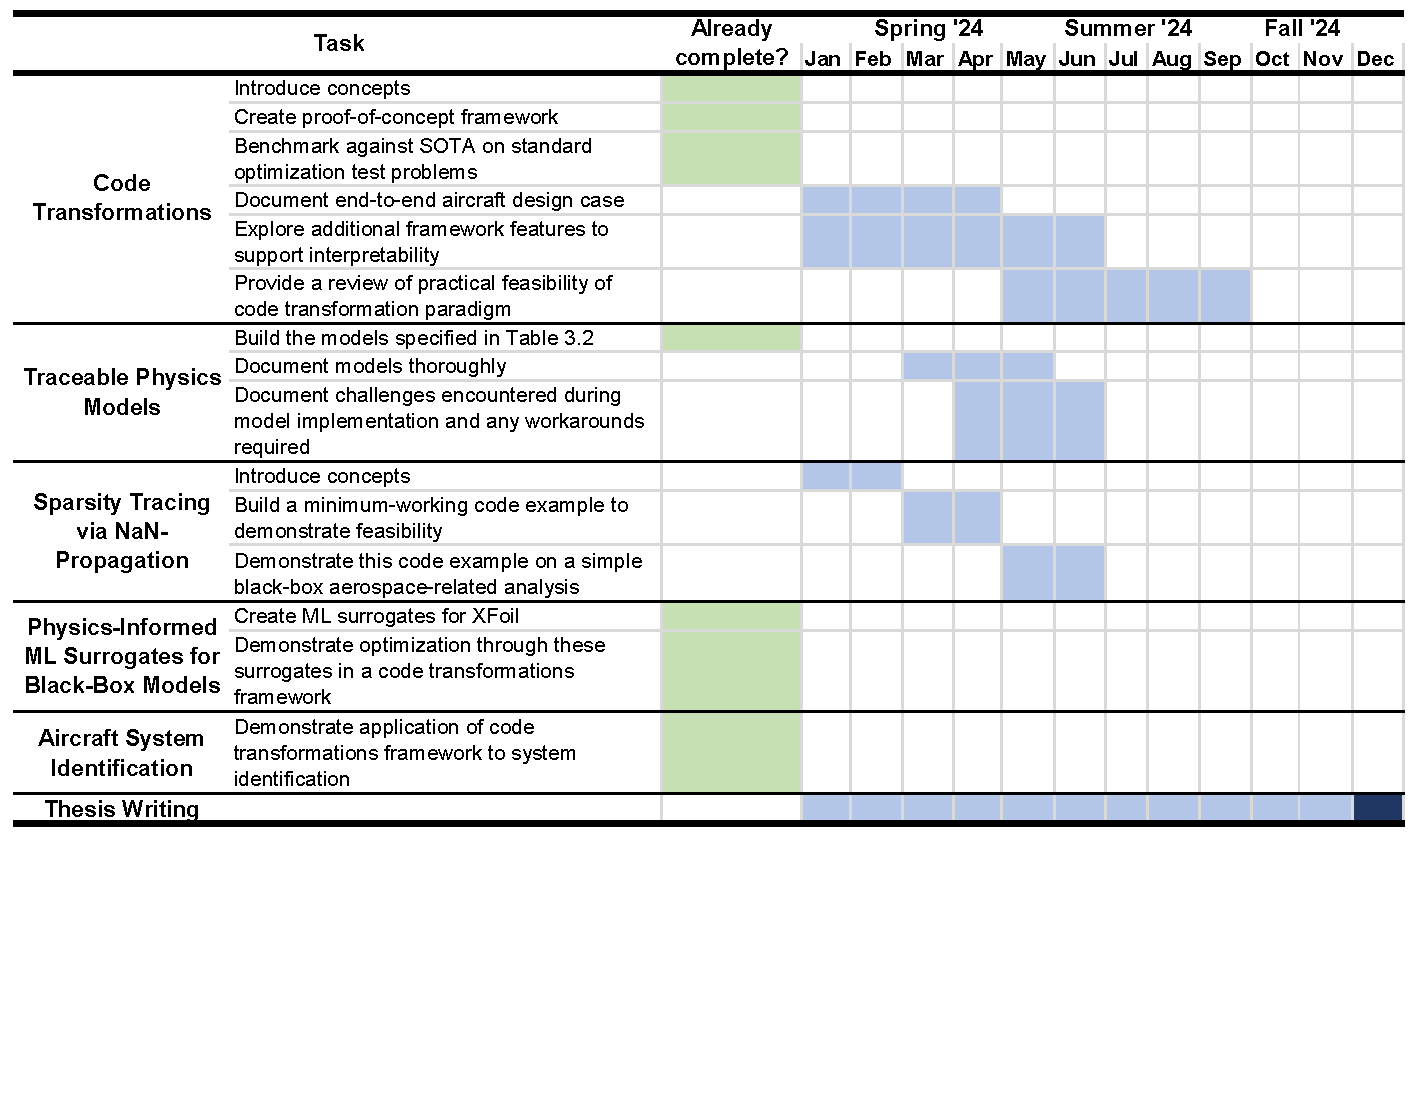
\includegraphics[width=\textwidth]{../figures/timeline.pdf}
        \label{tab:research_timeline}
    \end{table}


%    \include{timeline}

%
%    \subsection*{Spring 2024}
%
%    \begin{enumerate}
%        \item Motivate the optimization framework developed in the thesis.
%        \begin{enumerate}
%            \item Identify or develop an aircraft design benchmark problem suitable for comparing existing frameworks and their associated paradigms. The design problem should be realistic (incorporating all core aircraft disciplines), but it should not be overly complex. Potential suitable problems could include:
%            \begin{itemize}[noitemsep]
%                \item \href{https://github.com/peterdsharpe/AeroSandbox/blob/master/tutorial/02%20-%20Design%20Optimization/03%20-%20Aircraft%20Design%20-%20SimPleAC.ipynb}{SimPleAC}, a small aircraft design problem initially proposed by Warren Hoburg \cite{hoburg_geometric_2014} and further refined by Berk Ozturk \cite{ozturk_conceptual_2018}.
%                \item The solar seaplane design problem developed and implemented as part of TA work for MIT 16.821 in Spring 2023 \cite{solar_seaplane}.
%                \item An aircraft design problem adapted from the \href{https://www.aiaa.org/get-involved/students-educators/Design-Competitions}{AIAA Graduate Aircraft Design Competition}, where the 2023-24 problem is a self-launching electric sailplane.
%                \item Long-haul liquid-hydrogen-powered transport aircraft design, which was studied and developed for MIT 16.886 in Fall 2022 and MIT 16.885 in Fall 2023 \cite{gaubatz_estimating_2023, transport_aircraft}.
%            \end{itemize}
%%            (e.g., the NASA Common Research Model) and more realistic problems (e.g., the D8.8). The goal is to have a set of problems that can be used to evaluate the framework's performance across a range of problem sizes and complexities.
%            \item Implement the benchmark problem in several frameworks that are representative of state-of-the-art and/or industry-standard paradigms: AeroSandbox, OpenMDAO, GPkit, and a ``optimizer wrapped around black-box analysis'' method\footnote{Typical of industry methods, such as those seen in the development of the Facebook HALE aircraft development effort\cite{fbhale}}.
%            \item Compare the implementations on the basis of the three framework-level metrics identified in Section \ref{sec:code_transformations}: runtime speed, problem implementation speed, and mathematical flexibility. Document this thoroughly. Use this exercise as a jumping-off point to write a thesis chapter on how specific framework design choices affect each of these three metrics.
%            \item Show that the thesis framework makes large-scale optimization practical to implement at the conceptual design stage.
%        \end{enumerate}
%        \item Quantitatively illustrate the performance benefit associated with large-scale optimization in conceptual-level aircraft design:
%        \begin{enumerate}
%            \item Identify or develop an aircraft design benchmark problem suitable for comparing various levels of model fidelity at the conceptual design level. The design problem should be sufficiently complex such that it can be solved with or without the inclusion of secondary disciplines. Potential suitable problems could include:
%            \begin{itemize}[nolistsep]
%                \item MIT Firefly, a rocket-propelled micro-UAV design problem coupling packaging constraints, transonic aerodynamics, trajectory design, and propulsion design.
%                \item Dawn One, a high-altitude-long-endurance solar-powered aircraft.
%            \end{itemize}
%        \end{enumerate}
%    \end{enumerate}
%
%    \subsection*{Fall 2024}
%
%    \begin{enumerate}
%        \item Present the idea that implicit model assumptions and constraint-satisfaction information as ``metadata'' that should be % TODO
%    \end{enumerate}

    % TODO section


    \section{Facilities Required}
    \label{sec:facilities}

    No special facilities are required for this work beyond those already available at MIT AeroAstro.

    \begin{appendices}
        \chapter{Comparison of MDO Framework Paradigms}
        \label{chap:paradigm_comparison}

        This appendix aims to expand on the comparisons made in Table \ref{tab:paradigm_comparison} by providing more details on the pros and cons of various MDO paradigms. In this table, three qualitative metrics are defined over which MDO framework paradigms are evaluated. These metrics represent framework needs derived from the barriers to industry adoption that are identified in Chapter \ref{chap:literature}. Here, we define those metrics more precisely:

        \begin{enumerate}
            \item \textbf{Ease of implementation:} How much effort is required to implement a typical aircraft design problem (from ``concept idea'' to ``working code'') in this paradigm? How much optimization or programming expertise is required, beyond the basics needed to write engineering analysis code?
            \item \textbf{Computational speed and scalability:} How fast is the resulting design optimization problem to run, and how does this scale with problem size and number of disciplines? Are there other fundamental limits to scaling up analysis fidelity?
            \item \textbf{Mathematical flexibility:} What kinds of restrictions are present on the mathematical form of the optimization problem? This has important follow-on effects for backwards-compatability, as highly-restrictive frameworks preclude the use of existing engineering code and instead require from-scratch rewrites.
        \end{enumerate}

        From here, we can provide some notes on how various MDO paradigms are assessed:

        \subsection*{Black-Box Optimization}

        Black-box optimization refers to the common industry approach of taking an existing performance analysis toolchain and wrapping it in an optimizer. An example of this is shown in Figure \ref{fig:nested}. Here, the user has a ``black box'' function that takes in a vector of design variables and outputs a scalar objective and a vector of constraints. The user then wraps this function in an optimizer, without providing any other information (e.g., gradient or sparsity) about the function. The moniker ``black box'' refers to the fact that the internal workings of this analysis function are essentially opaque to the optimizer.

        \begin{figure}[H]
            \centering
            \includesvg[width=0.8\textwidth]{../figures/nested.svg}
            \caption{A representation of a traditional ``black-box'' wrapped-optimization approach, which remains the dominant MDO paradigm used by industry practitioners today. Figure adapted from \cite{drela_simultaneous_2010}.}
            \label{fig:nested}
        \end{figure}

        The main benefit of this approach is its conceptual simplicity: a black-box optimization paradigm tends to map most directly onto the ``mental model'' of optimization that most practicing engineers have. In this mental model, the forward problem (i.e., analysis) is the basis, and an inverse solve (i.e., optimization) is bolted on afterwards to wrap this. Because of this, black-box optimization is assessed to have the easiest path to implementation in industry. Modeling flexibility is likewise excellent due to the minimal information required by the optimizer.

        However, this approach has some drawbacks, which we enumerate here:
        \begin{enumerate}
            \item Computational performance invariably degrades rapidly as the number of design variables is increased. If a gradient-free optimizer is used, this is due to the curse of dimensionality, where the size of the feasible set of the design space grows exponentially with the number of design variables. with a gradient-based optimizer, scaling is better, but it still falls sharply behind more advanced paradigms due to the bottleneck of gradient computation via finite differencing.
            \item Convergence issues may exist if the wrapped analysis requires internal closure loops to be satisfied. If a wrapped analysis cannot achieve closure (i.e., feasibility) with a given set of inputs, the optimizer receives essentially no information that allows it to recover from this; this can render the optimization process brittle. Likewise, these closure loops can be inefficient -- lots of computational effort is spent closing iterative feasibility loops early in the design process, when the design is far from optimal.
            \item Finally, the black-box optimization approach typically forces a functional coding style (i.e., a callable data structure with defined inputs and outputs) in order to interface with an external optimizer. This can be unnatural to read and write, as engineers typically write analysis code in a procedural style. While simple analyses may allow easy conversion between functional and procedural coding styles, this task becomes substantially harder for larger codebases split across multiple files or modules.
        \end{enumerate}

        Because of these reasons, the runtime speed and scalability of black-box optimization methods is deemed relatively poor.

        \subsection*{Gradient-based with Analytic Gradients}

        Gradient-based optimization methods that are manually augmented with user-provided analytic gradients offer substantial runtime performance improvements over black-box optimization methods -- indeed, to-date this is the dominant approach in deep MDO methods where runtime speed is the primary limitation \cite{martins_coupledadjoint_2005}. However, deriving and implementing derivatives for each model can be a Herculean effort that is challenging to scale to wide MDO methods with hundreds of constituent models \cite{brelje_multidisciplinary_2021}. Moreover, this process requires significant end-user expertise and is often tedious and error-prone. Indeed, erroneous gradient calculations can be some of the most persistent and difficult errors to detect and debug \cite{martins_engineering_2021}. Due to the user expertise and engineering time required to implement each model in such a framework, this paradigm faces an uphill battle for conceptual design in industry.

        Modeling flexibility is approaches the total freedom that black-box optimization affords, although the requirement for differentiability (more precisely, $C^1$-continuity) can preclude certain types of conditional logic that do not preserve this. In practice, limitations due to this restriction are rare and can usually be worked around.

        \subsection*{Disciplined Optimization Paradigm}

        Disciplined optimization methods, such as geometric programming or convex programming methods, offer the ease-of-use of black-box optimization methods with the runtime speed of gradient-based methods with analytic gradients \cite{gpkit, kirschen}. Moreover, they carry notable additional benefits by virtue of their convex formulation: no initial guesses are required, and any optimum must be a global one.

        These benefits are achieved by restricting the space of mathematical operators, which limits the models that can be implemented into such a framework. Because of this restriction, model flexibility is scored low. Fortunately, geometric programming maps relatively well onto many sizing relations found in aircraft conceptual design, since many of these are power-law-like relations \cite{hoburg_geometric_2014}. However, even in conceptual aircraft design relations, a substantial number of exceptions to GP-compatibility exist, and this can be labor-intensive to resolve \cite{tao_phd_thesis}. Furthermore, this model inflexibility leaves little ability to scale up the level of fidelity to include common mid-fidelity analysis elements like nonlinear systems of equations or integrators. For this reason, disciplined optimization methods are scored lower on scalability, although they are quite competitive on runtime speed when the nature of the problem allows it to be compatible with such a framework.

        \subsection*{Code Transformations}

        On the metric of ease-of-implementation, code transformations are scored as identical to disciplined optimization paradigm. Both approaches allow a procedural modeling-language-like approach that tends to map closely onto existing engineering analysis code. Optimization components, like the variables, constraints, and objective, can be specified in natural-language syntax. Both are scored slightly below black-box optimization methods, since they both require understanding of certain paradigm-specific concepts. (In the case of disciplined optimization methods, this is convexity or GP-compatibility. In the case of code transformations, this is traceability.)

        Code transformations offer runtime speeds that equals or exceed those of dedicated disciplined optimization solvers on relevant problems. This paradigm also offers a pathway to medium-fidelity analysis that is often not possible with disciplined optimization methods. However, code transformations are relatively memory-hungry due to the storage of a complete computational graph; this precludes the high-fidelity analyses (e.g., RANS CFD) that are possible in an analytic-gradient paradigm. Likewise, hand-derived gradients can implement accelerations that are not yet possible with code transformations, such as more aggressive sparsity accounting, subtractive cancellation, and common subexpression elimination \cite{casadi, martins_complexstep_2003, martins_engineering_2021}. For these reasons, runtime speed and scalability falls somewhere between that of disciplined optimization methods and gradient-based methods with analytic gradients.

        Finally, modeling flexibility is vastly improved over disciplined optimization methods, as the only fundamental requirement is that of $C^1$-continuity, similar to that of other gradient-based methods. However, mathematical operators should be drawn from a set of pre-defined primitives \cite{ rackauckas_generalizing_2021}, which has the potential to reduce modeling flexibility if the numerics framework does not make appropriate syntax choices to mitigate this \cite{jax}. For these reasons, flexibility is assessed as slightly below that of gradient-based methods with analytic gradients.

    \end{appendices}

    % Bibliography
    \clearpage % or \cleardoublepage
    \addcontentsline{toc}{chapter}{Bibliography}
    \bibliography{../TeX/main, C:/Users/peter/Documents/Zotero/library, C:/Users/peter/Documents/Zotero/library-zotero}
    \bibliographystyle{ieeetr}


\end{document}